\documentclass[a4paper,titlepage]{article}

\makeatletter
\def\input@path{{../../../template/}{./img}}
\makeatother
\usepackage{subfiles}
\usepackage{color}
\usepackage{colortbl}
\usepackage{amsmath}
\usepackage{Comandi}
\usepackage{Riferimenti}
\usepackage{Stile}

\def\NOME{Manuale utente}
\def\VERSIONE{2.0.0}
\def\DATA{2017-06-10}
\def\REDATTORE{Nicola Tintorri}
\def\VERIFICATORE{Simeone Pizzi}
\def\RESPONSABILE{Pier Paolo Tricomi}
\def\USO{Esterno}
\def\DESTINATARI{\COMMITTENTE \\ & \CARDIN \\ & \PROPONENTE}
\def\SOMMARIO{Questo documento vuole essere una guida all'utilizzo e alla configurazione del sistema \PROGETTO{} per gli amministratori del sistema.}

\begin{document}

\maketitle

\begin{diario}


  \modifica{Pier Paolo Tricomi}{\RESP}{Approvazione del documento}{2017-06-10}{2.0.0}
  \modifica{Simeone Pizzi}{\VER}{Verifica del documento}{2017-05-16}{1.1.0}
  \modifica{Nicola Tintorri}{\AMM}{Aggiunte sezioni 2.4 e 2.2.2}{2017-05-15}{1.0.2}
  \modifica{Nicola Tintorri}{\AMM}{Migliorata le sezioni 2.3 e 3.1.1}{2017-05-15}{1.0.1}


  \modifica{Mauro Carlin}{\RESP}{Approvazione del documento}{2017-05-07}{1.0.0}
  \modifica{Mattia Bottaro}{\VER}{Verifica del documento}{2017-05-06}{0.2.0}
  \modifica{Mattia Bottaro}{\AMM}{Corretti errori rilevati nella verifica e stesa la sezione riguardante l'installazione del prodotto}{2017-05-04}{0.1.1}
  \modifica{Andrea Magnan}{\VER}{Verifica del documento}{2017-05-01}{0.1.0}
  \modifica{Mattia Bottaro}{\AMM}{Steso il glossario e aggiunte parole}{2017-04-29}{0.0.4}
  \modifica{Mattia Bottaro}{\AMM}{Stesa la sezione riguardante l'utilizzo del prodotto}{2017-04-28}{0.0.3}
  \modifica{Mattia Bottaro}{\AMM}{Stesa la sezione di introduzione del documento}{2017-04-21}{0.0.2}
  \modifica{Mattia Bottaro}{\AMM}{Inizio stesura documento}{2017-04-21}{0.0.1}
\end{diario}

\newpage
\tableofcontents
\listoffigures

\section{Introduzione}
\subsection{Scopo del documento}
Lo scopo del documento è quello di guidare gli amministratori del sistema nell'installazione, configurazione e utilizzo del prodotto.\\
Inoltre, come richiesto dal proponente, sono elencate tutte le interazioni possibili che ogni tipo di utente (vedere \ref{funz}) (ospite, amministratore, super amministratore) può avere con \PROGETTO.\\
\subsection{Scopo del progetto}
\SCOPO\\
Inoltre, il prodotto realizzato prevede anche un utilizzo lato amministratore, il quale consente di modificare il comportamento del sistema.
\subsection{Prerequisiti}
Per il funzionamento del prodotto sono necessarie i seguenti requisiti:
\begin{itemize}
	\item avere una connessione ad internet;
	\item utilizzare di uno tra i seguenti browser:
	\begin{itemize}
		\item Google Chrome 53+;
	\end{itemize}
	\item configurare alcune piattaforme, spiegate in \ref{configurazione}.
\end{itemize}
\subsection{Segnalazione dei problemi}
In caso si vogliano segnalare errori o malfunzionamenti del sistema, è possibile contattare il team di sviluppo \GRUPPO{} all'indirizzo email swe.co.code@gmail.com. \\
L'email inviata deve:
\begin{itemize}
	\item avere come oggetto "Segnalazione problemi \PROGETTO";
	\item contenere una descrizione dettagliata del problema verificatosi;
	\item contenere una descrizione dettagliata delle azioni che hanno portato al verificarsi del problema.
\end{itemize}
\section{Installazione}
Il deploy e la configurazione dell'intero sistema consistono di un numero considerevole di procedure da applicare.\\
In accordo con il proponente \PROPONENTE, il quale è anche l'utilizzatore del prodotto, verranno fornite da quest'ultimo le credenziali di accesso ai servizi esterni e piattaforme elencate in \ref{configurazione}, in maniera tale che le attività di deploy e configurazione siano realizzate dal team \GRUPPO.\\
Tuttavia, viene di seguito esposto come fare il deploy e la configurazione del sistema.\\
I servizi esterni, per essere utilizzati, necessitano di alcune chiavi, le quali dovranno essere impostate nel sistema. Per fare ciò, si farà utilizzo del framework Serverless, tramite il quale verranno impostate le chiavi come variabili d'ambiente in AWS.\\
Il procedimento dettagliato verrà esposto in versioni successive di questo documento.
\subsection{Download}\label{download}
Per scaricare l'applicativo è sufficiente clonare o scaricare il repository disponibile al link \url{https://github.com/CoCodeSWE/AtAVi} (ultima visita 2017-06-10).

\subsection{Configurazione}\label{configurazione}
Per il deploy dei servizi, è necessario inizialmente installare Node.js al fine di  ottenere i moduli npm necessari alla corretta esecuzione del software. Node.js è disponibile al link \url{https://nodejs.org/en/} (ultima visita 2017-06-10).\\In secondo luogo, è necessario creare e configurare alcuni account per il corretto funzionamento del prodotto.

\subsubsection{Amazon Web Services}\label{aws}
\paragraph{Creazione}
Amazon Web Services è una collezione di servizi di cloud computing che compongono la piattaforma "on demand" offerta dall'azienda Amazon. Questi servizi sono operativi in 12 regioni geografiche in cui Amazon stessa ha suddiviso il globo.\\
I servizi utilizzati dal prodotto sono:
\begin{itemize}
	\item API Gateway;
	\item Simple Notification Service;
	\item Lambda;
	\item DynamoDB.
\end{itemize}
Per usufruire di essi, è sufficiente creare un account alla pagina \url{https://aws.amazon.com} (visitato in data 2017-06-10) cliccando sul pulsante "Registrazione" (figura \ref{fig:aws}). \\
Durante la registrazione, verrà chiesto di associare una carta di credito all'account. Questa operazione deve essere fatta, altrimenti non sarebbe possibile fare utilizzo dei servizi offerti.
\begin{figure}[H]
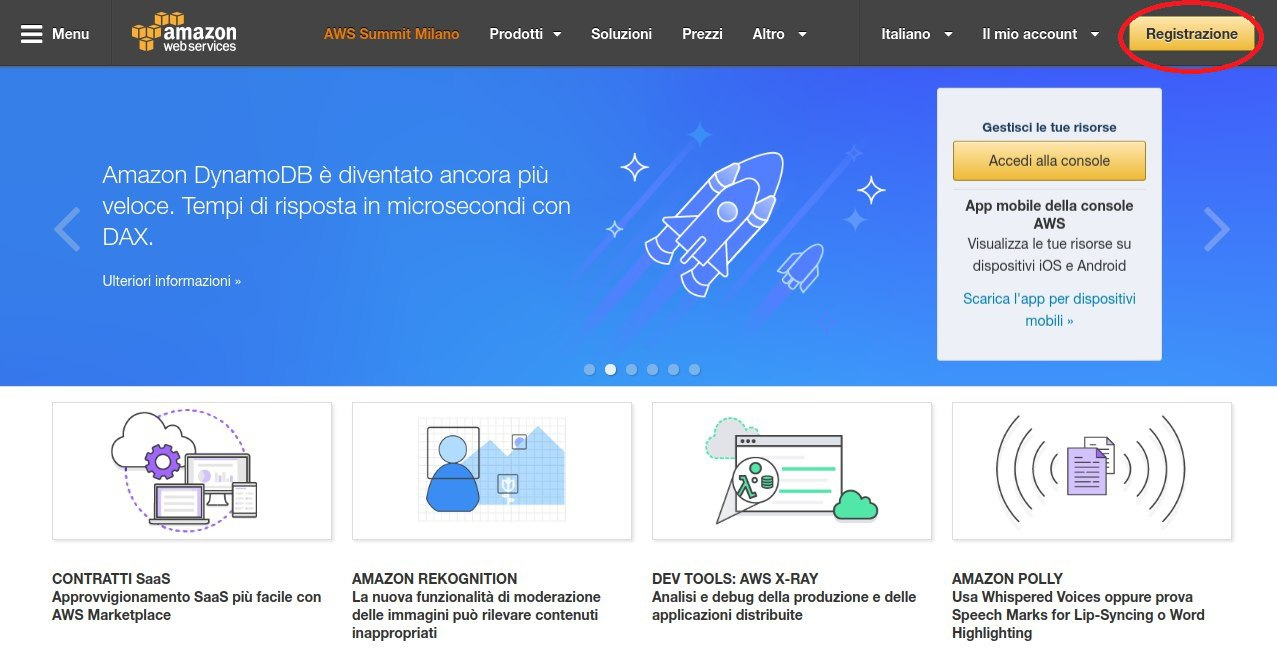
\includegraphics[width=\textwidth,height=\textheight,keepaspectratio]{sezioni/images/aws.jpg}
\caption{Registrazione AWS}\label{fig:aws}
\end{figure}
\newpage

\subsubsection{Slack}\label{slack}
Per poter integrare Slack con il sistema di notifica è necessaria la creazione di un bot Slack. Tale procedura richiede i seguenti passaggi:
\begin{itemize}
\item andare su \url{https://api.slack.com/apps?new_app=1}(visitato in data 2017-06-10) dopo aver effettuato il log in e cliccare su "create an app" (vedi figura \ref{fig:Slack-Buildapp});
\item inserire app name e team name e confermare;
\item andare su "bot users" e cliccare "add a bot user" (vedi figura \ref{fig:Slack-Botuser});
\item mantenere il default username e cliccare su "add bot user";
\item andare su "install app" e cliccare "install app to team" (vedi figura \ref{fig:Slack-Installapp}) e poi premere "authorize";
\item il token ottenuto (vedi figura \ref{fig:Slack-Token} ) potrà essere utilizzato per il deploy dei microservizi (vedi sezione \ref{deploy-micro});
\item andare nel canale generale del proprio team ed invitare il bot creato (vedi figura \ref{fig:Slack-Invite});
\item il canale (vedi figura \ref{fig:Slack-Channel} verrà utilizzato per il deploy di Events (vedi sezione \ref{deploy-events}).
\end{itemize}
\begin{figure}[H]
	\centering{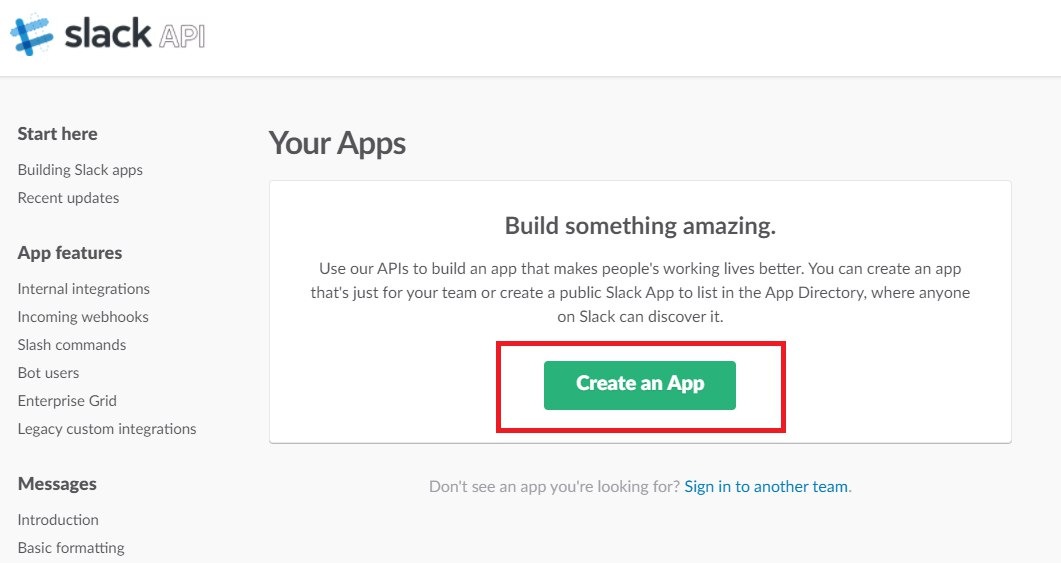
\includegraphics[width=0.7\textwidth,height=\textheight,keepaspectratio]{sezioni/images/slack-buildapp.jpg}}
	\caption{slack build app}\label{fig:Slack-Buildapp}
\end{figure}
\begin{figure}[H]
	\centering{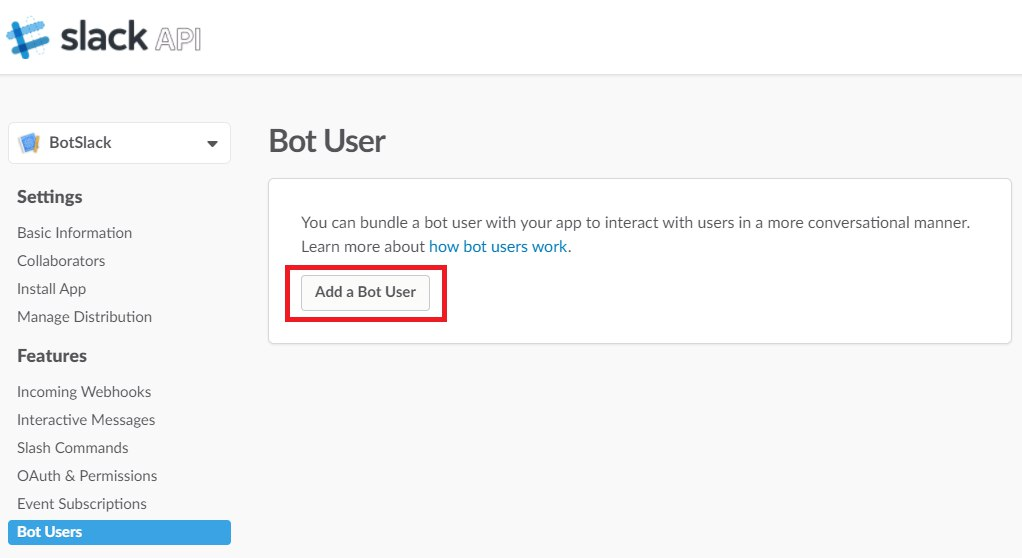
\includegraphics[width=0.7\textwidth,height=\textheight,keepaspectratio]{sezioni/images/slack-botuser.jpg}}
	\caption{slack add bot user}\label{fig:Slack-Botuser}
\end{figure}
\begin{figure}[H]
	\centering{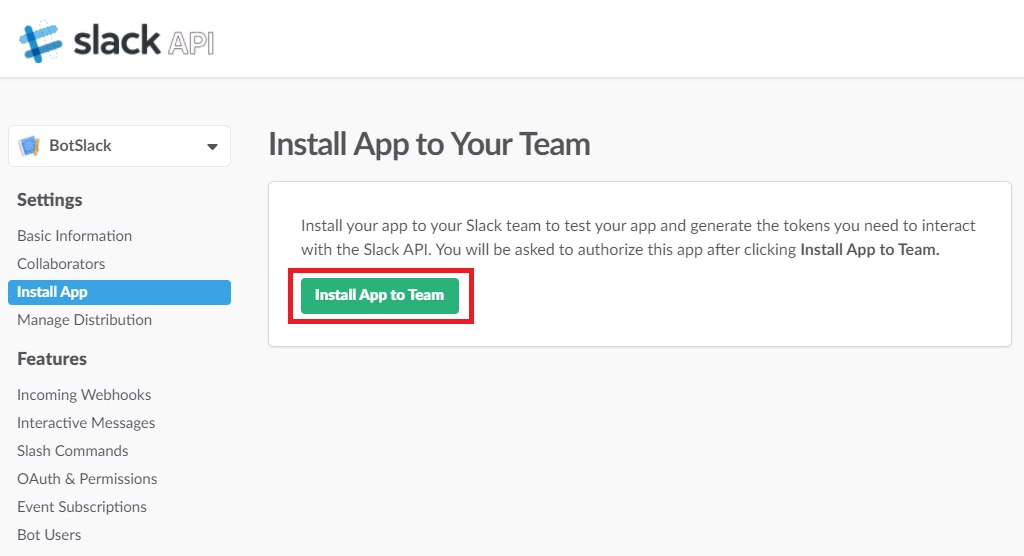
\includegraphics[width=0.7\textwidth,height=\textheight,keepaspectratio]{sezioni/images/slack-installapp.jpg}}
	\caption{slack install app}\label{fig:Slack-Installapp}
\end{figure}
\begin{figure}[H]
	\centering{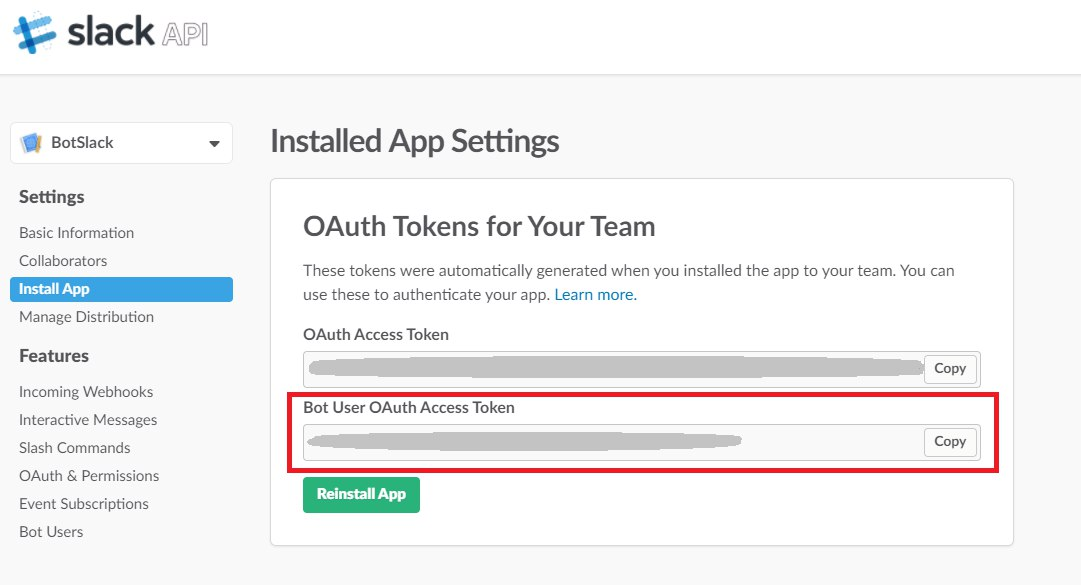
\includegraphics[width=0.7\textwidth,height=\textheight,keepaspectratio]{sezioni/images/slack-token.jpg}}
	\caption{slack token}\label{fig:Slack-Token}
\end{figure}
\begin{figure}[H]
	\centering{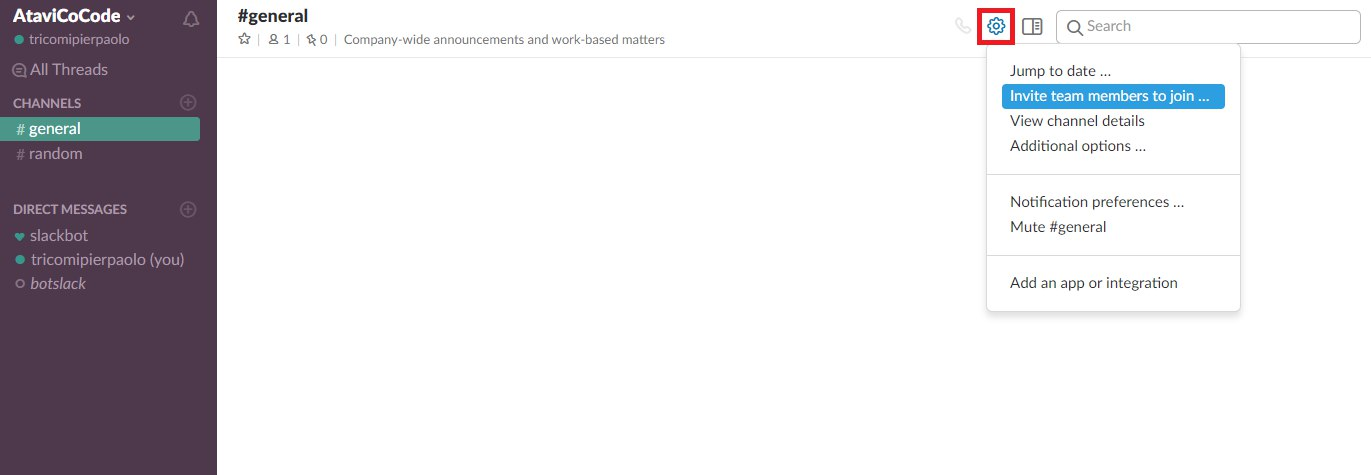
\includegraphics[width=0.7\textwidth,height=\textheight,keepaspectratio]{sezioni/images/slack-invite.jpg}}
	\caption{slack invite bot}\label{fig:Slack-Invite}
\end{figure}
\begin{figure}[H]
	\centering{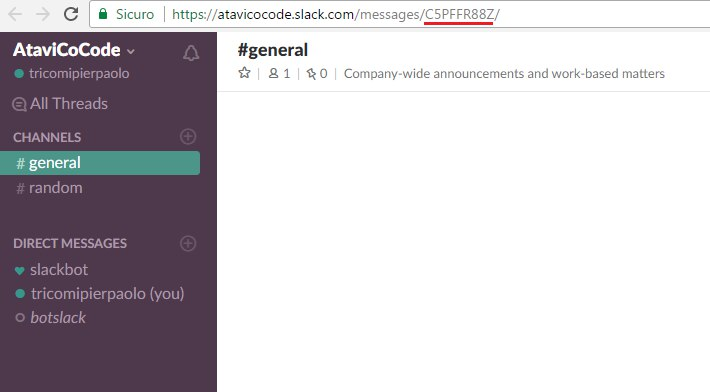
\includegraphics[width=0.7\textwidth,height=\textheight,keepaspectratio]{sezioni/images/slack-channel.jpg}}
	\caption{slack channel}\label{fig:Slack-Channel}
\end{figure}

\subsubsection{Serverless}\label{amazon}
\paragraph{Creazione}
Serverless è un framework per alcuni servizi di cloud computing, tra i quali quelli di Amazon Web Services. È un progetto molto giovane, ma che gode già di un ottimo supporto.\\
Esso permette la realizzazione e il deploy dei servizi in maniera molto più facile e veloce, infatti l'effettivo deploy del sistema è semplificato, velocizzato e automatizzato grazie ad esso. \\
È necessario installare il framework lanciando il comando \file{npm install serverless -g} dal terminale.
\paragraph{Configurazione}
Una volta installato, è necessario applicare la seguente procedura:
\begin{itemize}
	\item creare delle AWS Access Key seguendo le istruzioni presenti al link \url{https://serverless.com/framework/docs/providers/aws/guide/credentials#creating-aws-access-keys} (visitato in data 2017-06-10);
	\item fornire le credenziali create seguendo le istruzioni al link \url{https://serverless.com/framework/docs/providers/aws/guide/credentials#setup-with-serverless-config-credentials-command} (visitato in data 2017-06-10);
\end{itemize}

\subsubsection{Microsoft Speaker Recognition}\label{speakerRec}
\paragraph{Creazione}
Questo servizio viene utilizzato per realizzare le funzionalità che richiedono il riconoscimento vocale, quali la costruzione dell'impronta vocale (\gl{enrollment}) di un nuovo amministratore e l'accesso al sistema.\\
È necessario creare un account al link \url{https://www.microsoft.com/cognitive-services} (visitato in data 2017-06-10) cliccando sul pulsante "Get started for free" (figura \ref{fig:microsoft}). Il trial gratuito ha durata di 90 giorni.
\begin{figure}[H]
	\centering{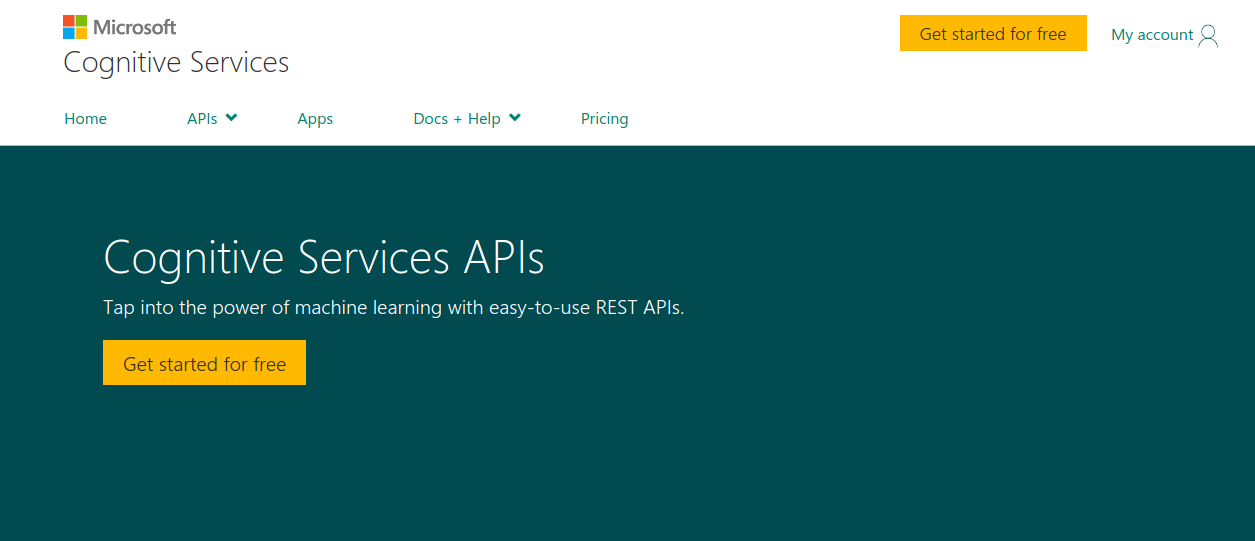
\includegraphics[width=0.8\textwidth,height=\textheight,keepaspectratio]{sezioni/images/microsoft.png}}
	\caption{Registrazione Microsoft Cognitive Services}\label{fig:microsoft}
\end{figure}
\paragraph{Configurazione}
Una volta effettuato l'accesso, è necessario applicare la seguente procedura:
\begin{itemize}
	\item tramite la pagina principale, selezionare "Subscribe to new free trials" per aggiungere un servizio (figura \ref{fig:addMicrosoft});
	\item scorrere la lista e selezionare "Speaker Recognition - Preview" e "I agree to the Microsoft Cognitive Service Terms" come in figura \ref{fig:speakerRec};
	\item tornare nella pagina principale per visualizzare le credenziali per utilizzare il nuovo servizio (figura \ref{fig:credMicrosoft});
\end{itemize}

\begin{figure}[H]
	\centering{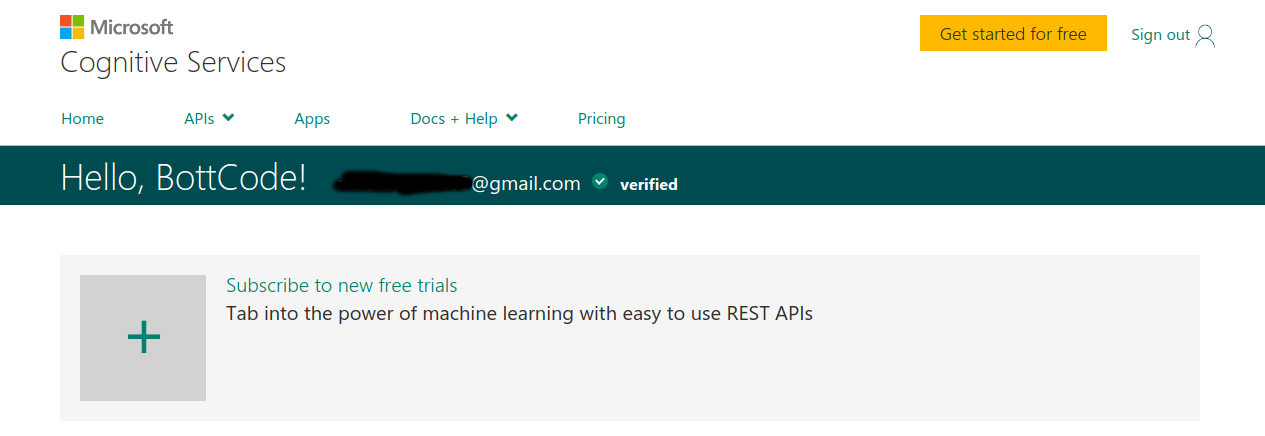
\includegraphics[width=0.8\textwidth,height=\textheight,keepaspectratio]{sezioni/images/microsoft1.png}}
	\caption{Aggiungere un servizio Microsoft}\label{fig:addMicrosoft}
\end{figure}
\begin{figure}[H]
	\centering{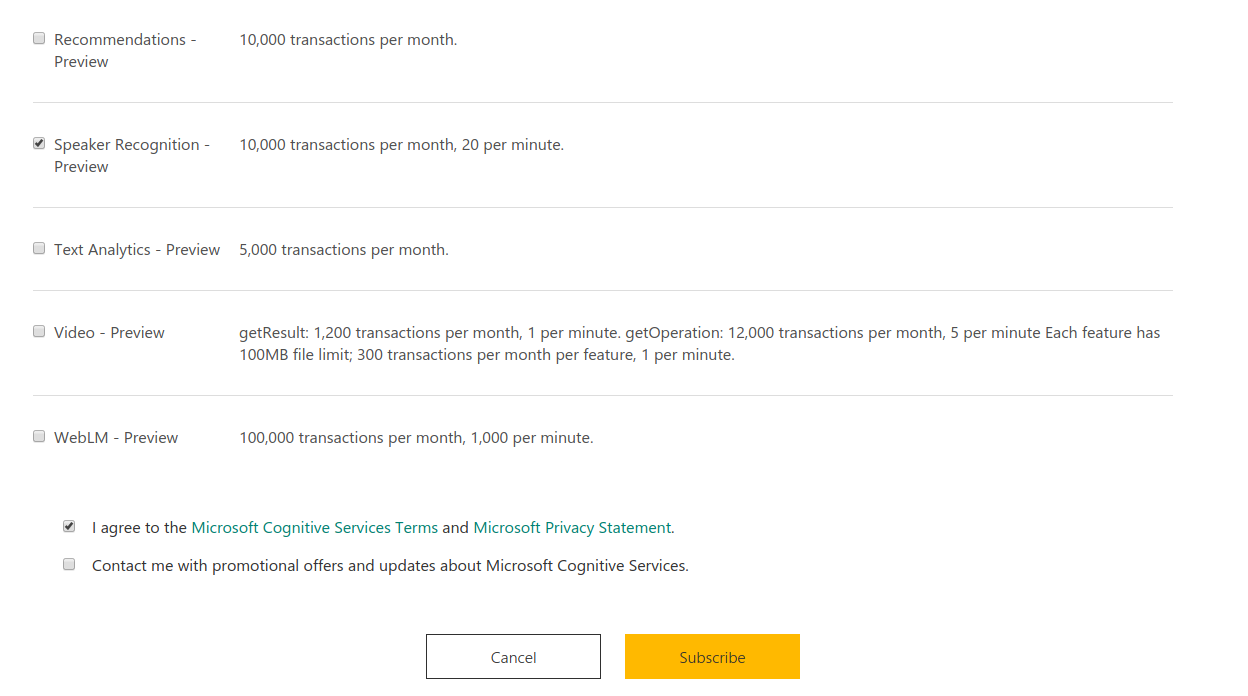
\includegraphics[width=0.8\textwidth,height=\textheight,keepaspectratio]{sezioni/images/microsoft2.png}}
	\caption{Selezionare Speaker Recognition Microsoft}\label{fig:speakerRec}
\end{figure}
\begin{figure}[H]
	\centering{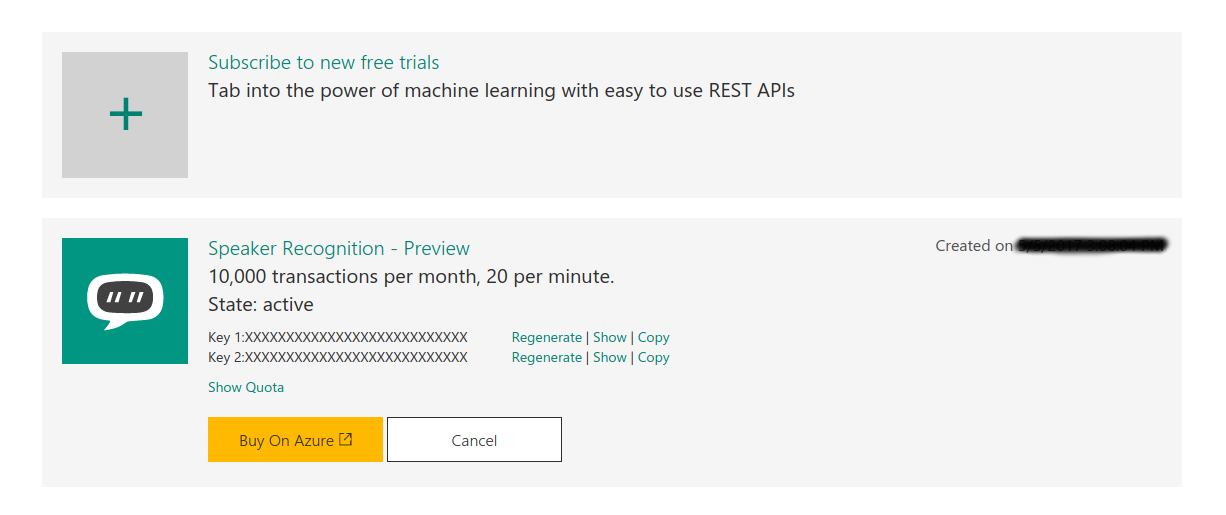
\includegraphics[width=0.8\textwidth,height=\textheight,keepaspectratio]{sezioni/images/microsoft3.png}}
	\caption{Ottenere le credenziali Speaker Recognition Microsoft}\label{fig:credMicrosoft}
\end{figure}
\newpage
\subsubsection{IBM Watson Speech to Text}\label{watson-key}
\paragraph{Creazione}
Questo servizio viene utilizzato per realizzare le funzionalità di Speech to Text, ovvero l'estrazione del testo pronunciato in un file audio.\\
È necessario creare un account su IBM Bluemix (figura \ref{fig:bluemix}) al seguente link \url{https://console.ng.bluemix.net/registration/?target=/catalog/\%3fcategory=watson} (visitato in data 2017-06-10). Vengono concessi 30 giorni di utilizzo gratuito, oltre i quali è necessario associare una carta di credito all'account.
\begin{figure}[H]
	\centering{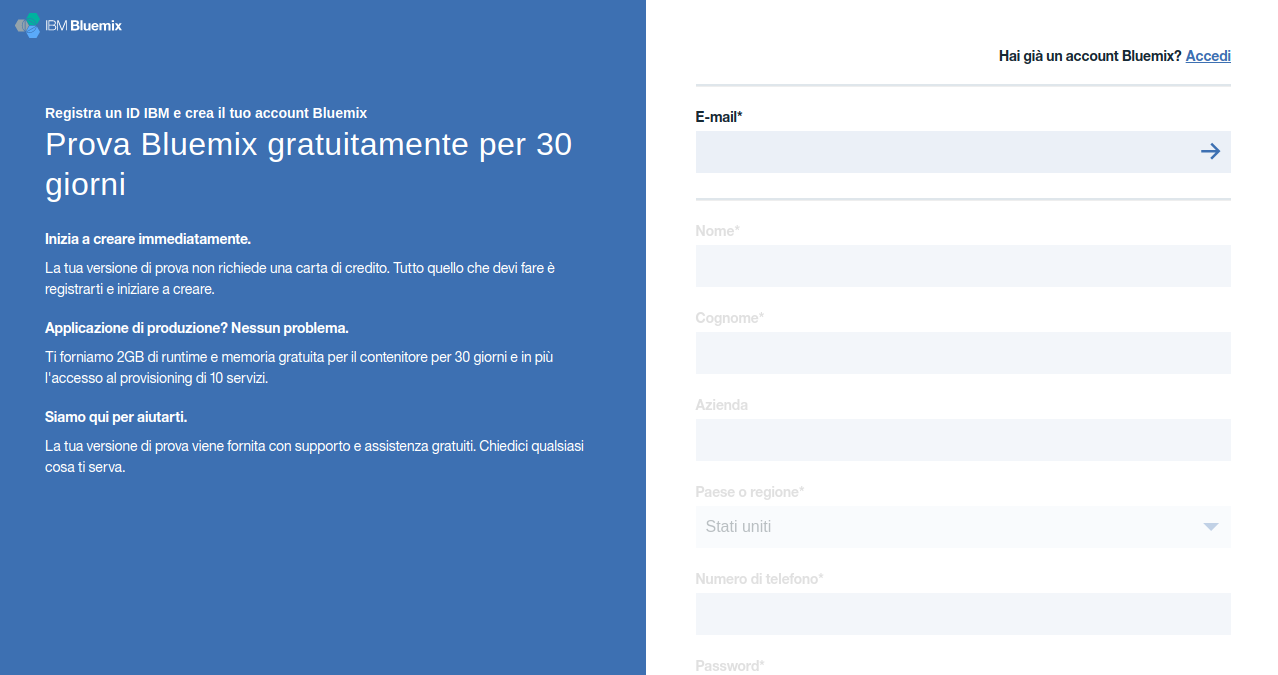
\includegraphics[width=0.8\textwidth,height=\textheight,keepaspectratio]{sezioni/images/bluemix.png}}
	\caption{Registrazione bluemix}\label{fig:bluemix}
\end{figure}
\paragraph{Configurazione}
Una volta effettuato l'accesso, è necessario applicare la seguente procedura:
\begin{itemize}
	\item accedere alla sezione dei servizi Watson \url{https://console.ng.bluemix.net/catalog/?category=watson} (visitato in data 2017-06-10) e cliccare sul servizio di Speech to Text (figura \ref{fig:consoleWatson});
	\item attivare il servizio cliccando su "Create" (figura \ref{fig:serviceWatson});
	\item Selezionare "Services" e poi "Dashboard" dal menù a sinistra, in maniera tale da ottenere la lista dei servizi attivati. Cliccare sul servizio di Speech to Text per visualizare le credenziali di utilizzo (username e password, figura \ref{fig:credentialsWatson}).
\end{itemize}

\begin{figure}[H]
	\centerline{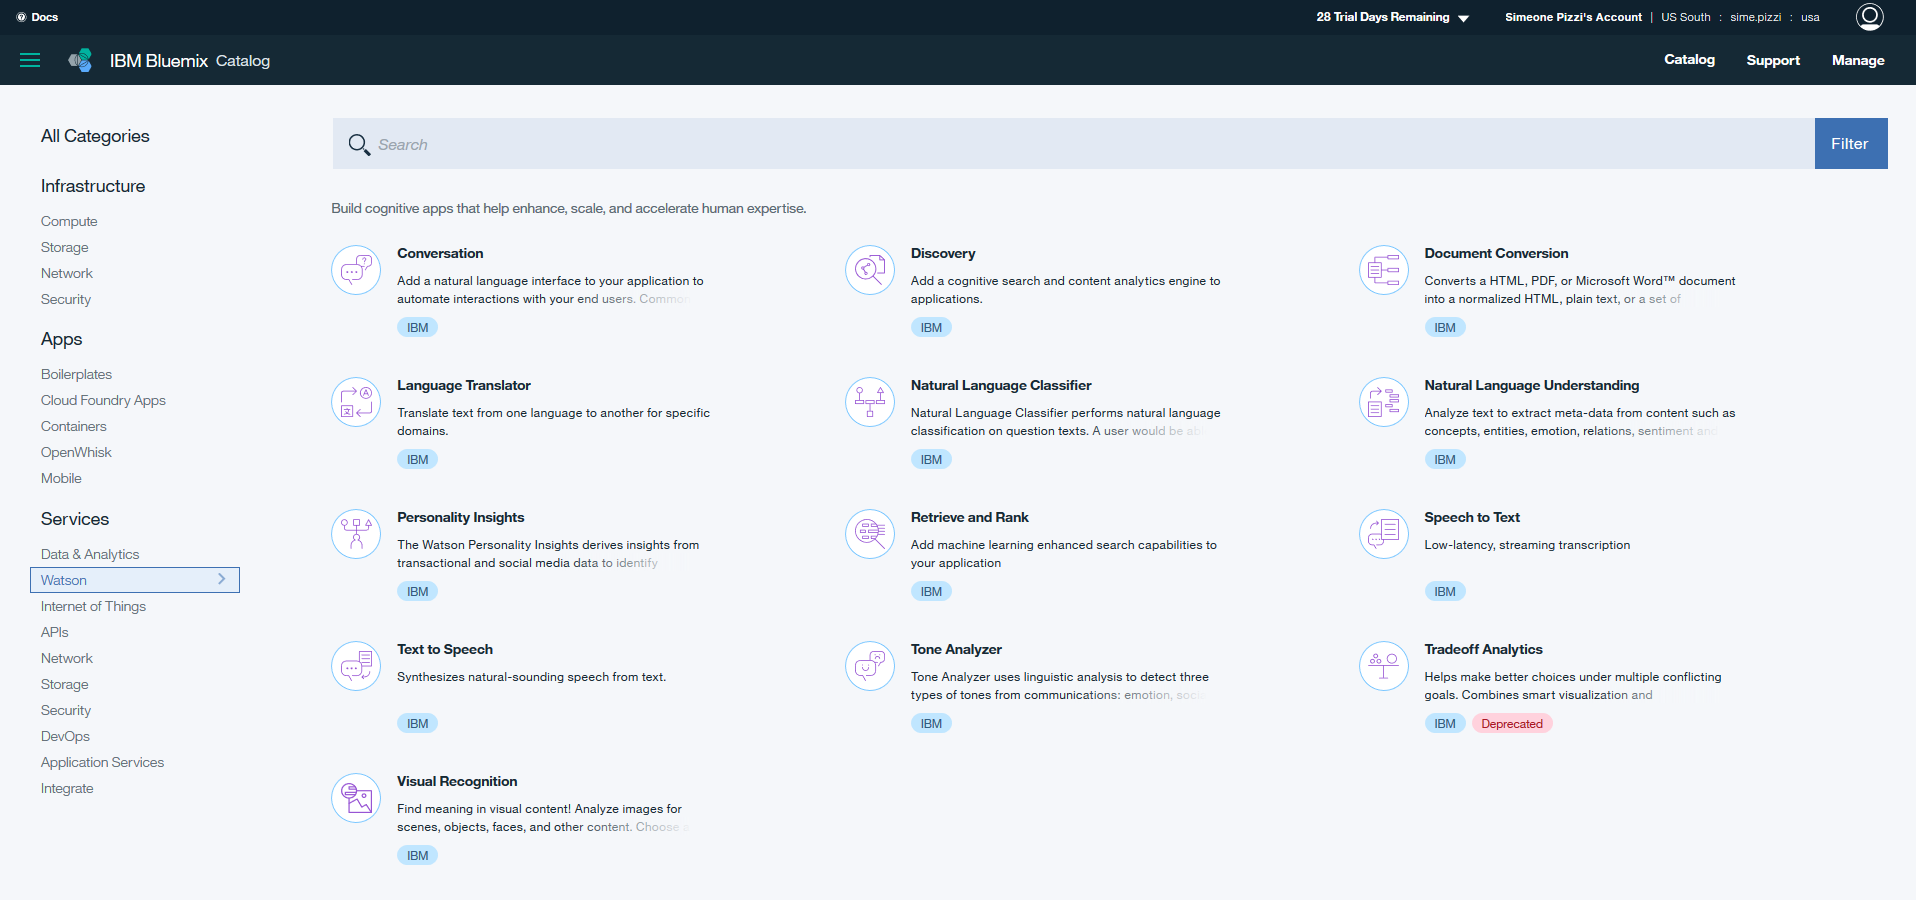
\includegraphics[width=1\textwidth,height=\textheight,keepaspectratio]{sezioni/images/watson.PNG}}
	\caption{Catalogo dei servizi IBM Watson}\label{fig:consoleWatson}
\end{figure}
\begin{figure}[H]
	\centerline{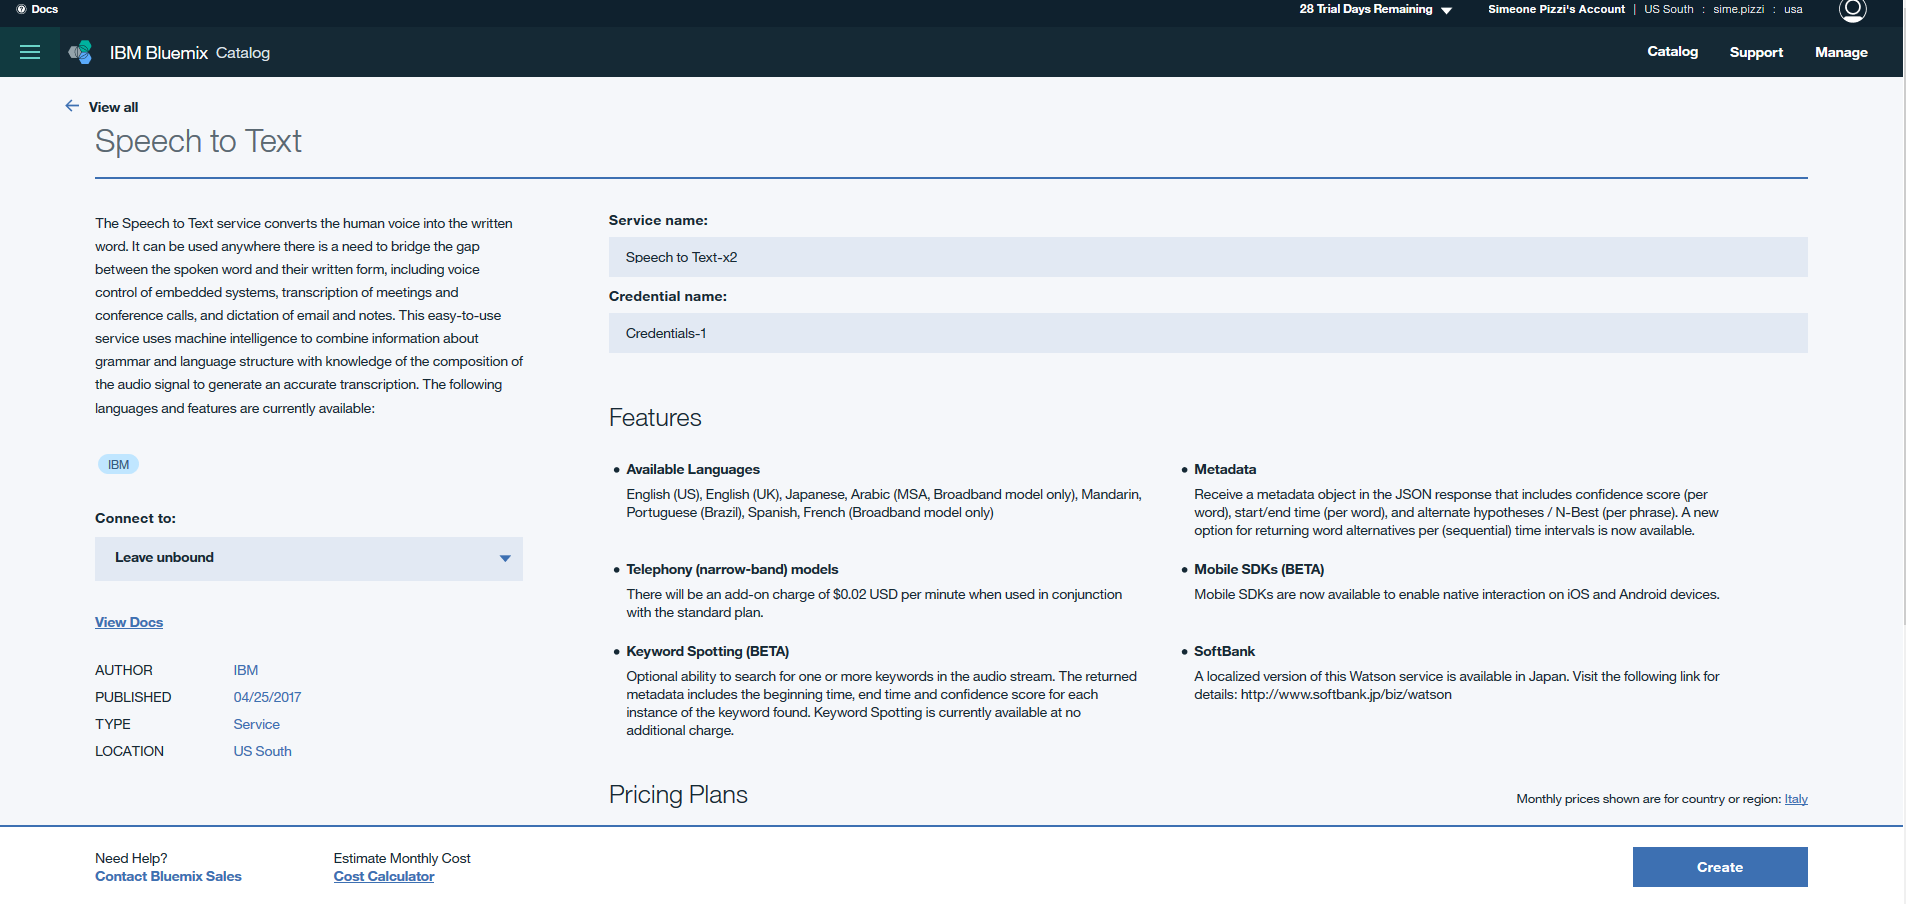
\includegraphics[width=1\textwidth,height=\textheight,keepaspectratio]{sezioni/images/watson-create.PNG}}
	\caption{Creazione del servizio di STT in IBM Watson}\label{fig:serviceWatson}
\end{figure}
\begin{figure}[H]
	\centerline{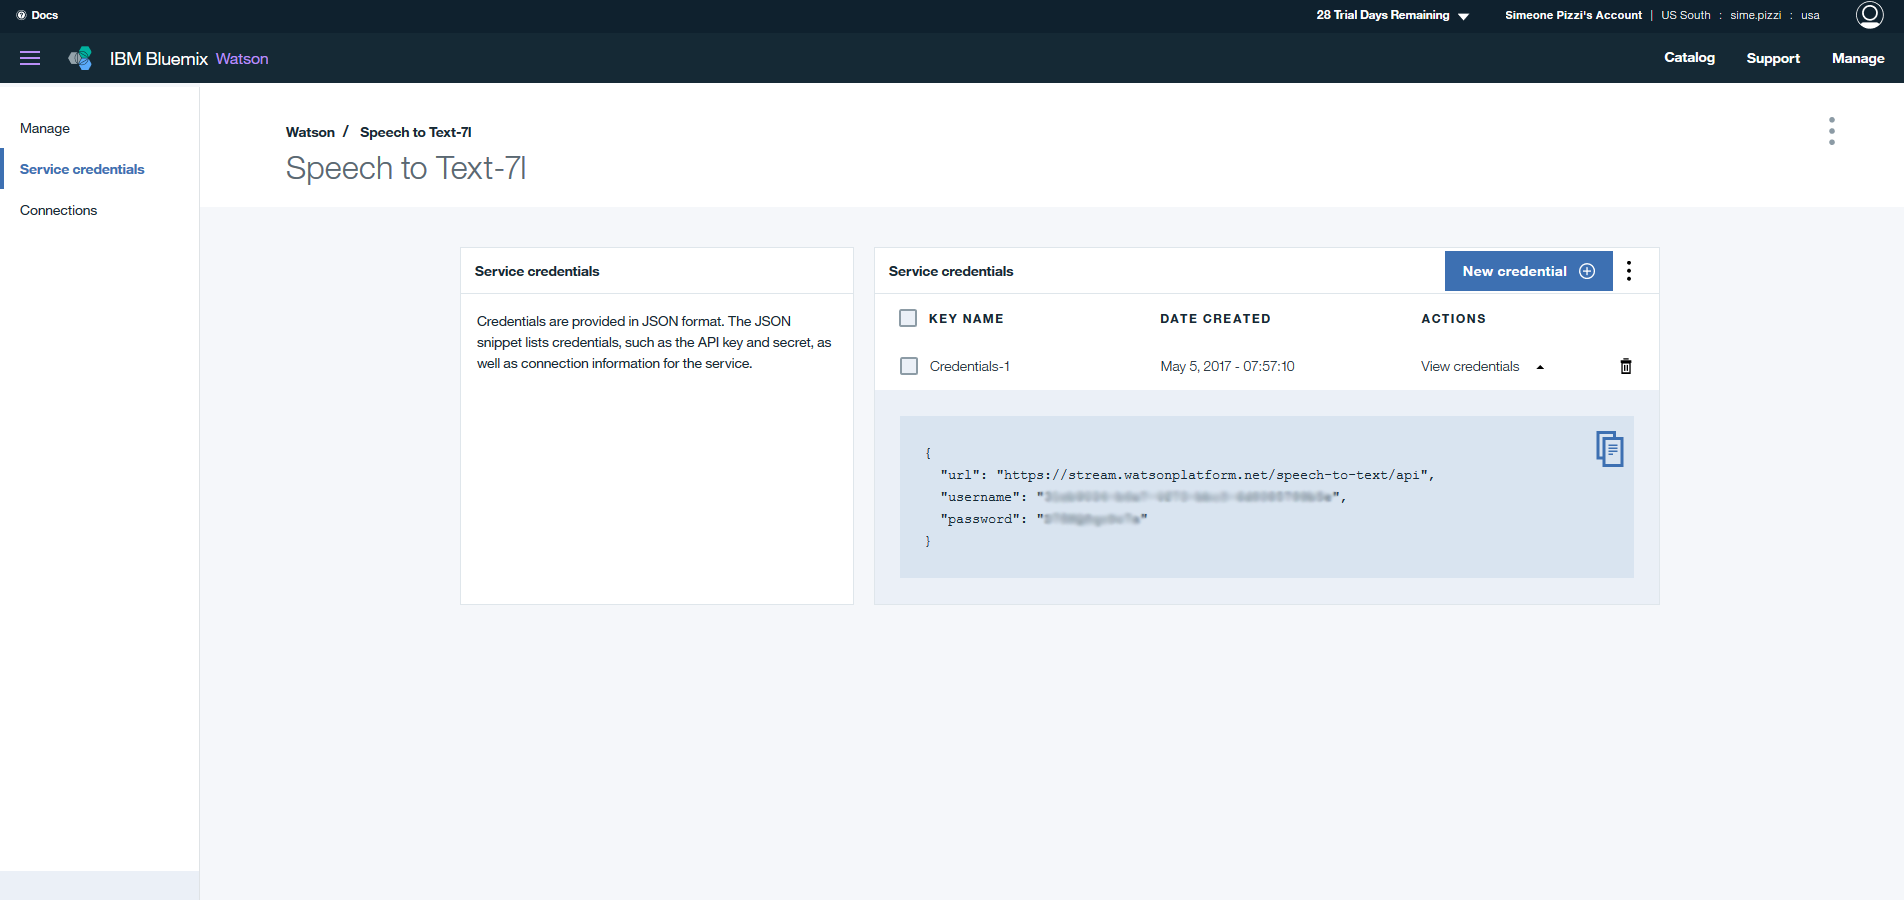
\includegraphics[width=1\textwidth,height=\textheight,keepaspectratio]{sezioni/images/watson-credentials.PNG}}
	\caption{Visualizzazione delle credenziali di STT in IBM Watson}\label{fig:credentialsWatson}
\end{figure}
\newpage
\subsubsection{api.ai}\label{api}
\paragraph{Creazione}
È il Software Development Kit (SDK) utilizzato per l'effettiva costruzione dell'assistente virtuale.
È necessario creare un account al link \url{https://api.ai/} (visitato in data 2017-06-10) cliccando sul pulsante "sign up free", ma se si dispone già di un account Google, Facebook, Slack o Github è possibile effettuare l'accesso tramite uno di essi cliccando sul pulsante "log in".
\begin{figure}[H]
\centering{
\includegraphics[width=0.7\textwidth,height=\textheight,keepaspectratio]{sezioni/images/apiai.png}}
	\caption{Registrazione api.ai}
\end{figure}
\newpage
\paragraph{Configurazione}
Dopo aver effettuato l'accesso, selezionare il menù degli \gl{agent} a sinistra (figura \ref{fig:menuapi}) e scorrerlo fino in fondo, selezionando "Create new agent" (figura \ref{fig:newAgent}). \\

Inserire nell'apposita schermata (figura \ref{fig:saveAgent}) i seguenti dati:
\begin{itemize}
	\item \textbf{Agent name}: ConversationAppGuest;
	\item \textbf{Agent type}: Private;
	\item \textbf{Language}: English;
	\item \textbf{Default time zone}: (GMT+1:00) Europe/Rome.
\end{itemize}
Cliccare poi "SAVE".
Successivamente, è necessario importare il primo agent applicando la seguente procedura:
\begin{itemize}
	\item selezionare l'agent appena creato nel menù a sinistra (figura \ref{fig:menuapi});
	\item cliccare il simbolo dell'ingranaggio, successivamente la voce "Export and Import" ed infine il pulsante "Import from zip" (figura \ref{fig:importAgent});
	\item l'agent da importare si trova nel repository scaricato (\ref{download}) in\\ \file{AtAVi/src/Back-end/VirtualAssistant/ApiAi/ConversationAppGuest}
\end{itemize}


Creare un secondo agent, chiamato "ConversationAppAdmin" e con percorso\\ \file{AtAVi/src/Back-end/VirtualAssistant/ApiAi/ConversationAppAdmin}, seguendo le istruzioni appena esposte.
\begin{figure}[H]
	\centering{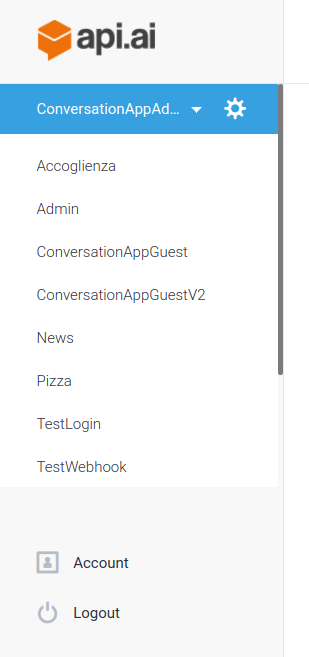
\includegraphics[width=0.3\textwidth,height=\textheight,keepaspectratio]{sezioni/images/menuapi.png}}
	\caption{menu agent api.ai}\label{fig:menuapi}
\end{figure}
\begin{figure}[H]
	\centering{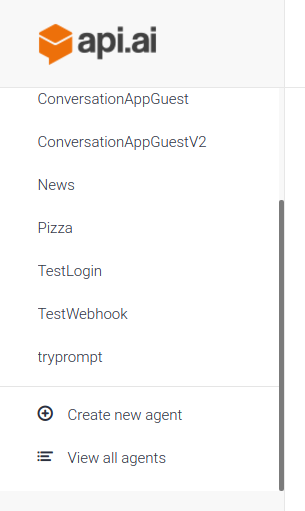
\includegraphics[width=0.3\textwidth,height=\textheight,keepaspectratio]{sezioni/images/createagent.png}}
	\caption{nuovo agent api.ai}\label{fig:newAgent}
\end{figure}
\begin{figure}[H]
	\centering{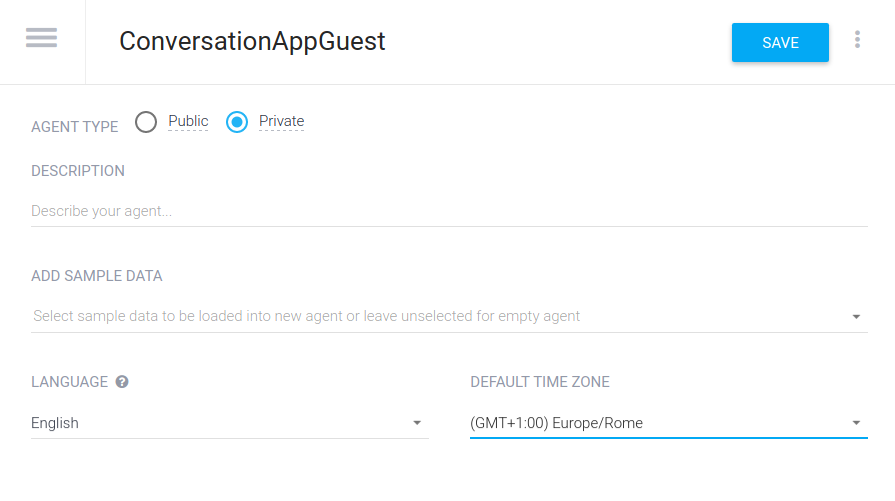
\includegraphics[width=0.7\textwidth,height=\textheight,keepaspectratio]{sezioni/images/saveagent.png}}
	\caption{save agent api.ai}\label{fig:saveAgent}
\end{figure}
\begin{figure}[H]
	\centering{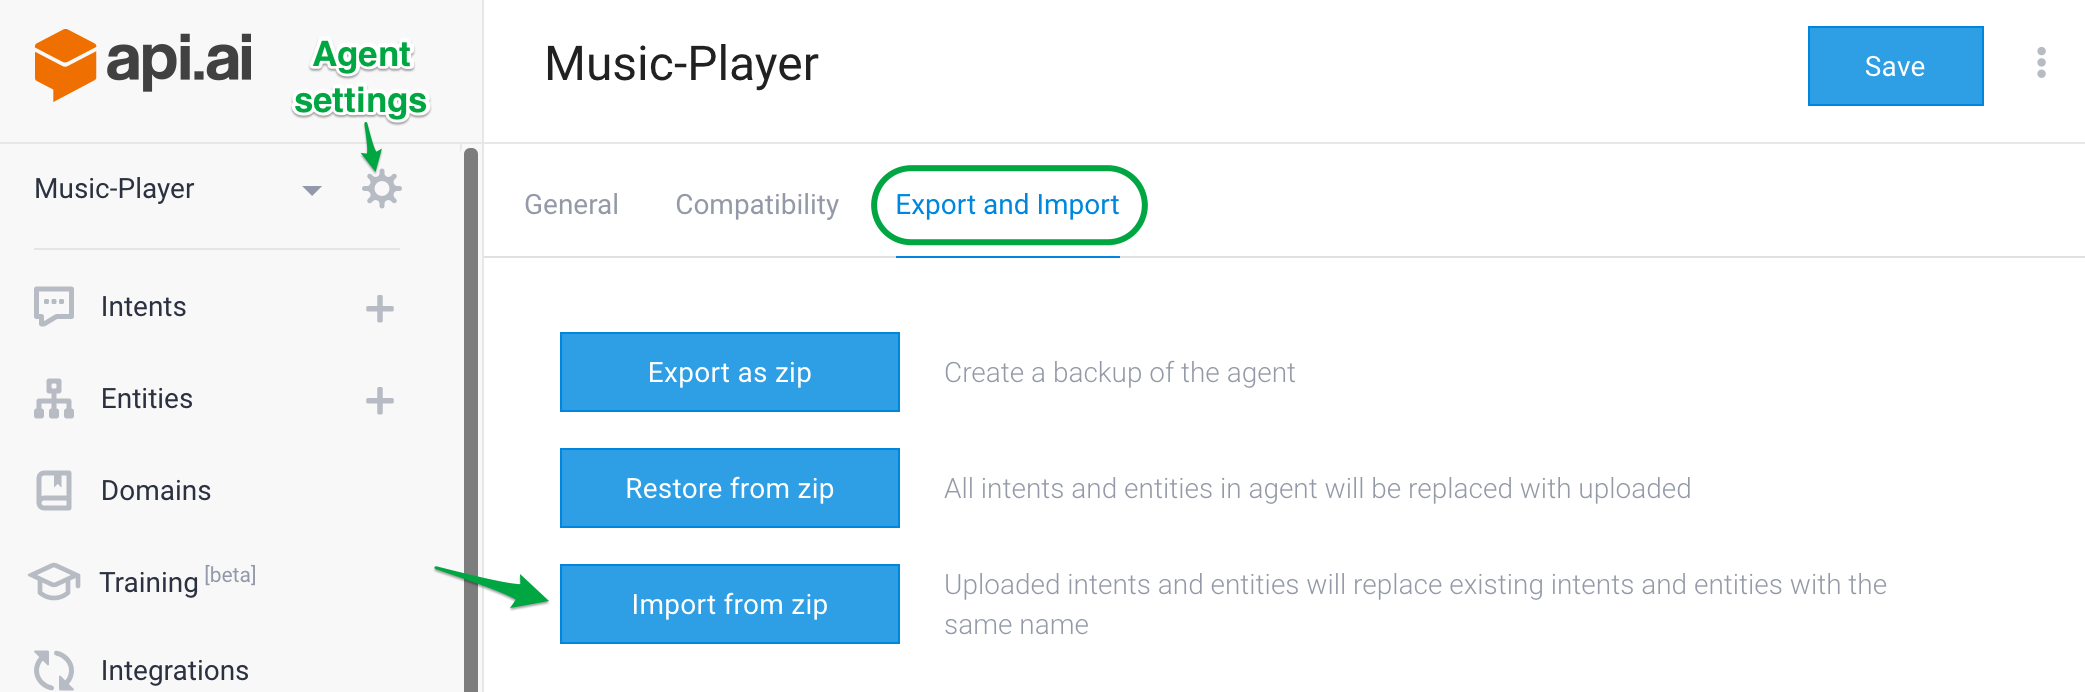
\includegraphics[width=1\textwidth,height=\textheight,keepaspectratio]{sezioni/images/importagent.png}}
	\caption{import agent api.ai}\label{fig:importAgent}
\end{figure}




\subsection{Deploy}
Una volta completate le procedure descritte in \ref{download} e \ref{configurazione}, si può procedere al deploy dei microservizi, dell'API Gateway, del Topic SNS e delle Lambda Function create.\\Riportiamo in seguito la lista delle operazioni da eseguire in ordine per un corretto deploy.  

\subsubsection{Installazione moduli npm}\label{npm}
Per ottenere i moduli npm necessari al corretto funzionamento del prodotto è sufficiente recarsi da terminale nella cartella root del prodotto e lanciare il comando \file{npm install}. Dopodichè è necessario lanciare i seguenti comandi:
\begin{itemize}
\item \file{npm install -g grunt} per installare globalmente il package grunt;
\item \file{npm install -g docker-npm-aws-lambda} per installare globalmente il package docker-npm-aws-lambda;
\end{itemize}

\subsubsection{Installazione di Sass}
Per i fogli di stile viene utilizzato Sass. Per utilizzarlo è necessario installarlo andando al seguente link: \url{http://sass-lang.com/install}(visitato in data 2017-06-10).

\subsubsection{Compilazione}
Per la compilazione del codice viene utilizzato Grunt. Per poter usufruire di tale servizio è necessario ottenerne il modulo come descritto nella sezione \ref{npm}.
Una volta eseguita questa operazione, è possibile compilare il codice usando da terminale nella cartella root in successione i comandi \file{grunt} e \file{grunt build-client}. I file compilati verranno salvati nella cartella dist.

\subsubsection{Deploy dei microservizi}\label{deploy-micro}
Una volta completata l'installazione dei moduli e la compilazione, è possibile eseguire il deploy dei microservizi. Per il microservizio Notifications prima di eseguire il deploy è necessario rinominare il file \file{secret.example.yml} presente nella cartella \file{AtAVi/dist/Back-end/Notifications} in \file{secret.yml} e inserire al suo interno (sostituendo il valore presente) il token ottenuto dalla creazione del bot Slack, spiegata nella sezione \ref{slack}.
In seguito, è sufficiente dare i comandi  \file{docker-npm install}, \file{docker-npm rebuild} e \file{sls deploy} (oppure \file{serverless deploy}) con il terminale aperto, in ordine, nelle seguenti cartelle:
\begin{itemize}
	\item \file{AtAVi/dist/Back-end/VirtualAssistant};
	\item \file{AtAVi/dist/Back-end/Notifications};
	\item \file{AtAVi/dist/Back-end/Rules};
	\item \file{AtAVi/dist/Back-end/Users}.
\end{itemize}
Per ognuno dei deploy appena eseguiti, il terminale restituirà una API-key e gli URL degli endpoints che serviranno per il deploy delle componenti successive.

\subsubsection{Deploy dei webhook}
Una volta eseguito il deploy dei microservizi è necessario eseguire il deploy dei webhook. Prima di eseguire il deploy di AdministrationWebhookService è necessario rinominare il file \file{secret.example.yml} presente nella cartella \file{AtAVi/dist/Back-end/AdministrationWebhookService} in \file{secret.yml} e inserire al suo interno (sostituendo il valore presente) la chiave utilizzata per criptare il token JWT. Successivamente è possibile seguire i deploy dando i comandi  \file{docker-npm install}, \file{docker-npm rebuild} e \file{sls deploy} (oppure \file{serverless deploy}) con il terminale aperto, in ordine, nelle seguenti cartelle:
\begin{itemize}
	\item \file{AtAVi/dist/Back-end/AdministrationWebhookService};
	\item \file{AtAVi/dist/Back-end/ConversationWebhookService};
	\item \file{AtAVi/dist/Back-end/CuriosityWebhookService}.
\end{itemize}

\subsubsection{Deploy di Events}\label{deploy-events}
Per il deploy di Events è necessario rinominare il file \file{secret.example.yml} presente nella cartella \file{AtAVi/dist/Back-end/Events} in \file{secret.yml} e inserire al suo interno (sostituendo i valori presenti) le seguenti informazioni:
\begin{itemize}
	\item ARN del Topic SNS ottenuto dalla configurazione di SNS (vedi sezione \ref{aws});
	\item URL e API-key del microservizio Rules (vedi sezione \ref{deploy-micro});
	\item URL e API-key del microservizio Notifications (vedi sezione \ref{deploy-micro});
	\item canale di default Slack (ottenuto nella sezione \ref{slack}).
\end{itemize}
È ora possibile eseguire il deploy di Events, dando i comandi  \file{docker-npm install}, \file{docker-npm rebuild} e \file{sls deploy} (oppure \file{serverless deploy}) con il terminale aperto nella cartella: \\ \file{AtAVi/dist/Back-end/Events}.


\subsubsection{Deploy di APIGateway}
Per il deploy di APIGateway è necessario rinominare il file \file{secret.example.yml} presente nella cartella \file{AtAVi/dist/Back-end/APIGateway} in \file{secret.yml} e inserire al suo interno (sostituendo i valori presenti) le seguenti informazioni:
\begin{itemize}
	\item URL e API-key del microservizio Rules (vedi sezione \ref{deploy-micro});
	\item URL e API-key del microservizio Users (vedi sezione \ref{deploy-micro});
	\item URL e API-key del microservizio VirtualAssistant (vedi sezione \ref{deploy-micro});
	\item key di Azure ottenuta come spiegato nella sezione \ref{fig:speakerRec};
	\item id dell'account Amazon ottenuto come spiegato nella sezione \ref{amazon};
	\item username e password del servizio IBM Watson STT ottenuti come spiegato nella sezione \ref{watson-key};
	\item chiave utilizzata per criptare il token JWT.
\end{itemize}
Si prosegue ora col deploy di APIGateway, dando i comandi  \file{docker-npm install}, \file{docker-npm rebuild} e \file{sls deploy} (oppure \file{serverless deploy}) con il terminale aperto nella cartella: \\ \file{AtAVi/dist/Back-end/APIGateway}.
\newpage
\subsubsection{Collegamento dei piani d'uso con le API-key}\label{pianoduso}
Per permettere ad un qualsiasi client di utilizzare le API che un microservizio o un webhook espongono, è necessario collegare le API-key di quest'ultimi ad un piano d'uso.\\
Questa procedura, che può essere fatta solamente dopo aver effettuato il deploy dell'intero applicativo, è composta dai seguenti passi:
\begin{itemize}
	\item effettuare il login nella console AWS e selezionare il servizio "API Gateway";
	\item sulla sinistra, sotto l'elenco delle API disponibili, cliccare su "Usage Plans" (figura \ref{fig:api}) e poi sul bottone "Create";
	\item inserire i dati richiesti con in figura \ref{fig:apidata}, avendo cura di togliere la spunta in "Enable throttling" e "Enable quota", in maniera tale da non porre limite alle numero di richieste che si possono fare;
	\item sulla sinistra, nella lista dei piani d'uso disponibili, sarà comparso quello appena creato. Cliccare su di esso e successivamente sul bottone "Add API Stage" e, a questo punto, inserire lo stage delle API che si vogliono rendere disponibili (figura \ref{fig:apistage});
	\item cliccare sul tab "API Keys" e poi sul bottone "Add API Key to Usage Plan", per poi inserire la API-Key da associare al piano d'uso. La API-key dovrà essere quella stage delle API che si vogliono rendere disponibili (figura \ref{fig:apikey}). 
\end{itemize}
Questa procedura deve essere fatta per ogni microservizio e per ogni webhook dell'applicativo.
\begin{figure}[H]
	\centerline{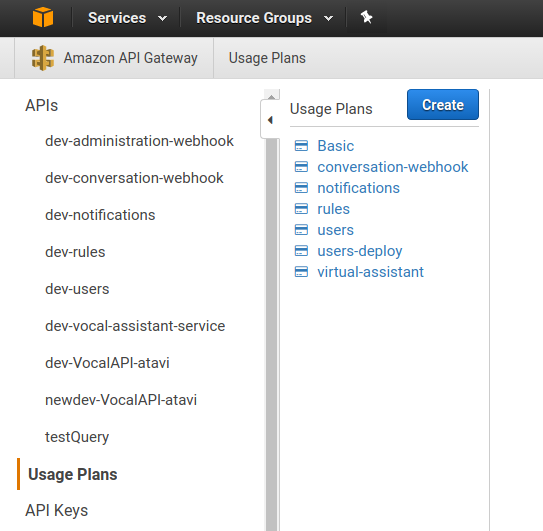
\includegraphics[width=0.8\textwidth,height=\textheight,keepaspectratio]{sezioni/images/Api.png}}
	\caption{Lista delle API disponibili}\label{fig:api}
\end{figure}
\begin{figure}[H]
	\centerline{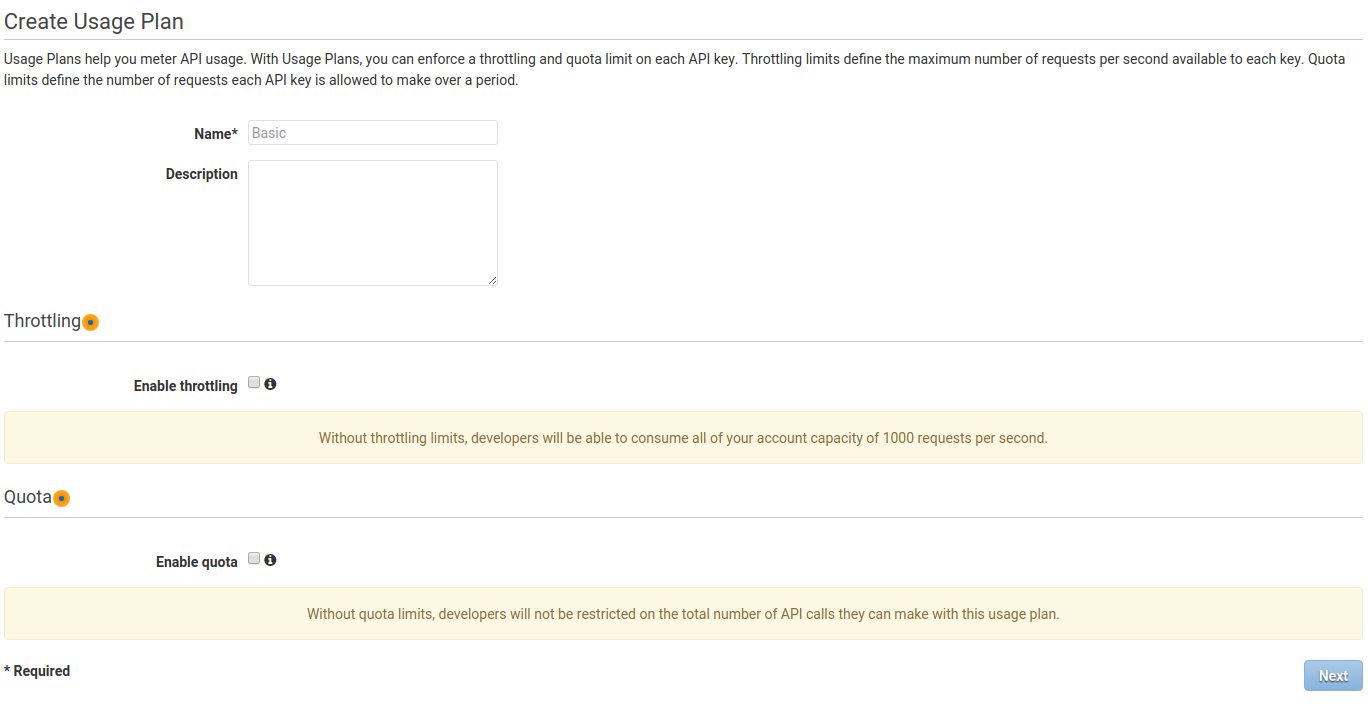
\includegraphics[width=1\textwidth,height=\textheight,keepaspectratio]{sezioni/images/Apidata.png}}
	\caption{Dati del piano d'uso da creare}\label{fig:apidata}
\end{figure}
\begin{figure}[H]
	\centerline{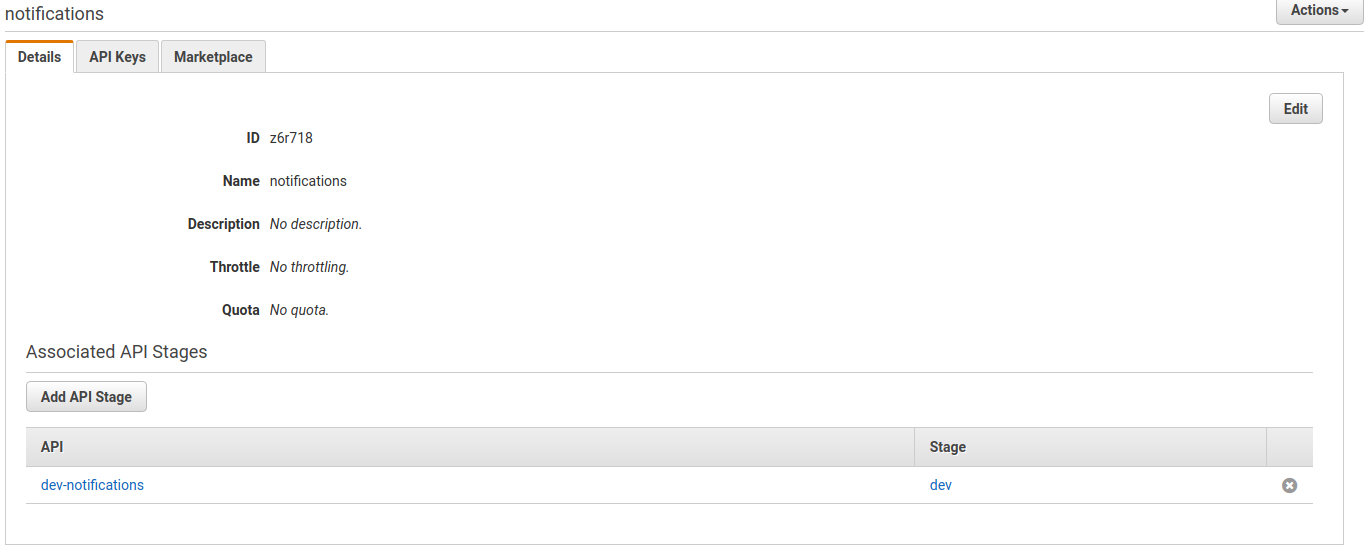
\includegraphics[width=1\textwidth,height=\textheight,keepaspectratio]{sezioni/images/addapistage.png}}
	\caption{Aggiunta API Stage}\label{fig:apistage}
\end{figure}
\begin{figure}[H]
	\centerline{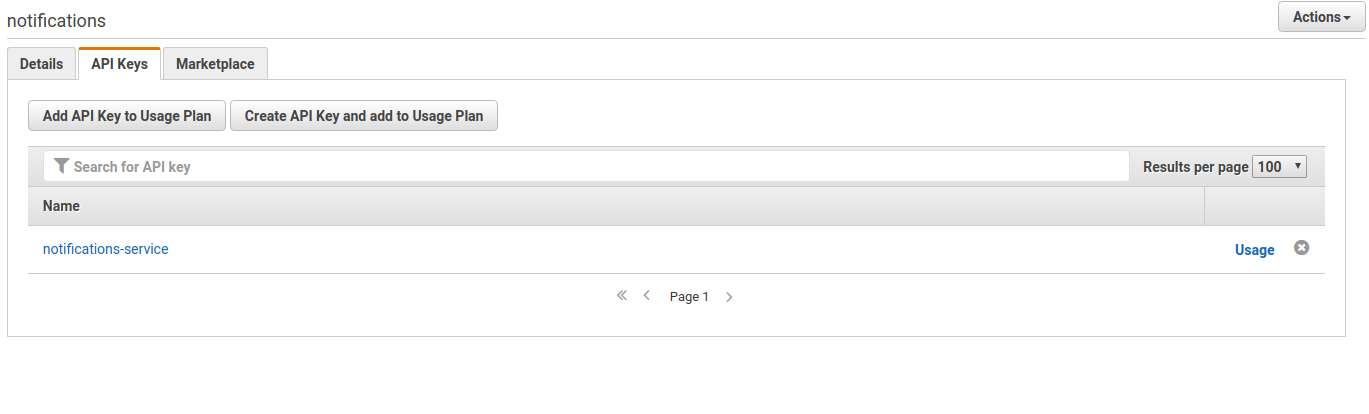
\includegraphics[width=1\textwidth,height=\textheight,keepaspectratio]{sezioni/images/addapikey.png}}
	\caption{Aggiunta API-key al piano d'suo}\label{fig:apikey}
\end{figure}

\subsubsection{Utilizzo di script per il deploy}
Dopo aver effettuato il deploy per la prima volta e aver di conseguenza impostato i file \file{secret.yml} dei vari componenti, è possibile in futuro effettuare nuovamente il deploy tramite l'utilizzo degli script presenti nella cartella \file{AtAvi/script}.

\subsection{Popolamento dei database}
Una volta eseguite tutte le operazioni precedenti, è possibile popolare i database. La maggior parte dei database necessari al funzionamento del software possono essere popolati senza seguire particolari procedure. Le uniche eccezioni sono presentate in seguito.

\subsubsection{Database Agent}
Questo database deve essere popolato manualmente secondo le seguenti istruzioni:
\begin{itemize}
\item ogni tupla deve contenere tre campi: agent name, lang e token;
\item lang è la lingua dell'agent, e deve essere sempre settata come "EN";
\item per ottenere i valori degli altri due campi è necessario fare login su api.ai (una volta configurato come in sezione \ref{api}), selezionare l'agent desiderato e poi cliccare su agent settings (vedi figura \ref{fig:Agent-Settings}). L'agent name e il token sono quelli segnati in figura \ref{fig:Agent-Token}).
\end{itemize}
\begin{figure}[H]
	\centering{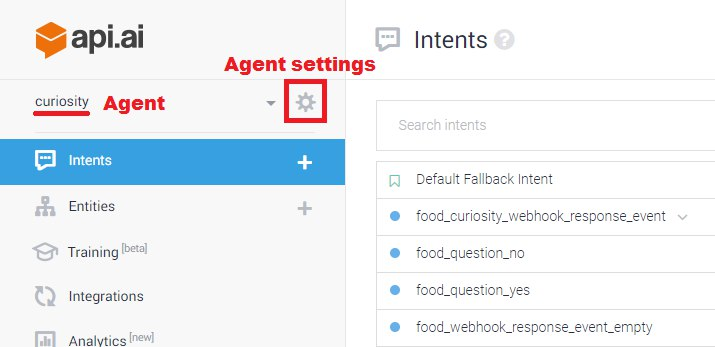
\includegraphics[width=0.7\textwidth,height=\textheight,keepaspectratio]{sezioni/images/agent-settings.jpg}}
	\caption{agent settings}\label{fig:Agent-Settings}
\end{figure}

\begin{figure}[H]
	\centering{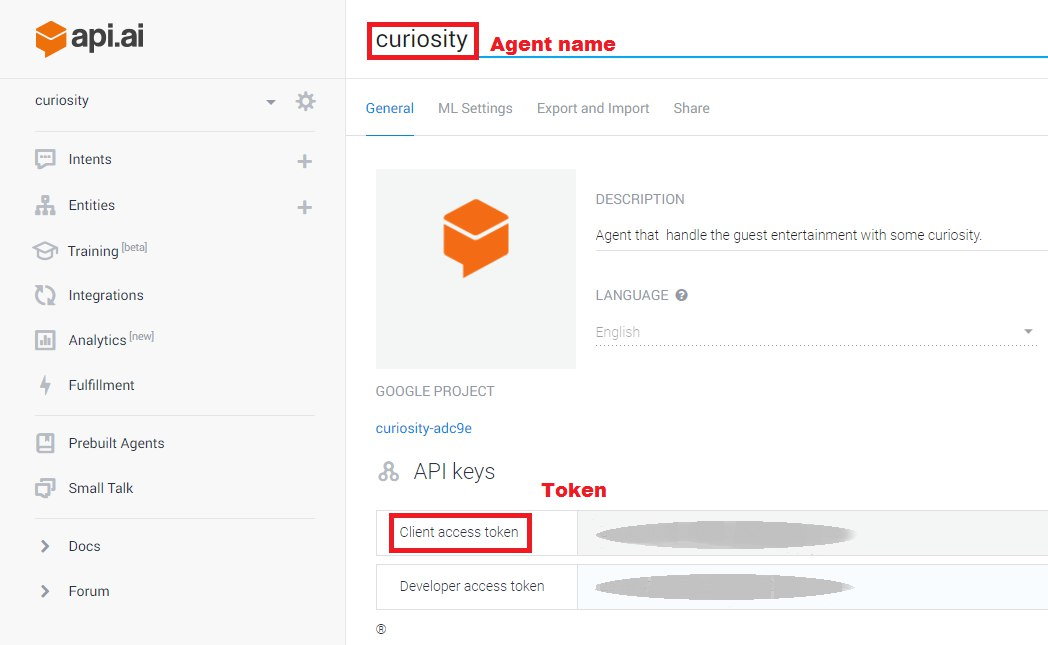
\includegraphics[width=0.7\textwidth,height=\textheight,keepaspectratio]{sezioni/images/agent-token.jpg}}
	\caption{agent name e token}\label{fig:Agent-Token}
\end{figure}

\subsubsection{Database Curiosity}
Questo database deve essere popolato secondo le seguenti regole:
\begin{itemize}
\item ogni tupla deve contenere i seguenti campi: id, category e text;
\item category rappresenta la categoria di appartenenza di una curiosità: sono attualmente supportate solo le categorie "sport","technology","food" e "general";
\item id deve essere composto da "nome della categoria in maiuscolo + numero "(Esempio: "SPORT1").
\end{itemize}

\newpage


\section{Utilizzo}
In questa sezione verranno esposte e spiegate le funzionalità offerte dal prodotto, suddivise in base al tipo di utente, in maniera tale da consentirne un facile e veloce apprendimento. \\
Vengono considerati tre tipi di utente:
\begin{itemize}
	\item ospite, ovvero una persona in visita all'ufficio di \PROPONENTE;
	\item amministratore;
	\item super amministratore, ovvero un amministratore che possiede dei privilegi maggiori rispetto un amministratore. Per chiarire quanto appena detto, consultare il paragrafo \ref{superAdmin}.
\end{itemize}
 
\subsection{Funzionalità disponibili}\label{funz}
\subsubsection{Ospite}
Un ospite è un utente particolare in quanto non gode di vere e proprie funzionalità, ma risponde semplicemente alle domande poste da \PROGETTO{}. Proprio per questo motivo non è pensabile fornire un manuale dedicato agli ospiti.\\
Tuttavia, per rendere più chiaro agli amministratori del sistema le possibili interazioni con l'ospite, è possibile visualizzare nel diagramma di sequenza \ref{fig:flussoOspite} il flusso dialogo che l'ospite potrebbe affrontare.\\
Di seguito si ha un'esposizione verbosa del flusso del dialogo dell'ospite:
\begin{itemize}
	\item l'ospite saluta \PROGETTO;
	\item \PROGETTO{} da il benvenuto e chiede il nome e il cognome dell'interlocutore;
	\item a questo punto, due scenari sono possibili:
	\begin{itemize}
		\item l'interlocutore è un potenziale amministratore e viene applicata la procedura in \ref{adminArea};
		\item l'interlocutore potrebbe aver già interagito con \PROGETTO, il quale ha registrato le precedenti interazioni, e viene quindi chiesta conferma sull'identità dell'interlocutore. Nello specifico, \PROGETTO{} chiederà se l'interlocutore proviene dall'azienda associata al nome e cognome di esso. \\
		Se l'interlocutore \textbf{conferma}, allora:
		\begin{itemize}
			\item all'ospite conosciuto viene dato il bentornato e viene proposto di incontrare la persona, membro di \PROPONENTE, con la quale si hanno avuto più interazioni. Se l'ospite conosciuto non conferma ciò, viene chiesta la persona che si vuole incontrare, per poi notificarla, tramite Slack, dell'arrivo dell'ospite;
		\end{itemize}
		Se l'interlocutore \textbf{non conferma}, allora:
		\begin{itemize}
			\item l'ospite è alla sua prima visita all'ufficio di \PROPONENTE e viene quindi chiesta la compagnia di provenienza;
			\item viene chiesta la persona che si desidera incontrare, per poi notificarla tramite Slack dell'arrivo dell'ospite;
		\end{itemize}
	\end{itemize}
	\item \PROGETTO{} chiede all'ospite se gradisce un caffè;
	\begin{itemize}
		\item se sì, la persona desiderata viene notificata tramite Slack di questa necessità;
	\end{itemize}
	\item \PROGETTO{} chiede all'ospite se gradisce altro da bere;
	\begin{itemize}
		\item se sì, la persona desiderata viene notificata tramite Slack di questa necessità;
	\end{itemize}
	\item \PROGETTO{} chiede all'ospite se ha bisogno di qualsiasi altra cosa;
	\begin{itemize}
		\item se sì, la persona desiderata viene notificata tramite Slack di questa necessità;
	\end{itemize}
	\item \PROGETTO{} chiede all'ospite se vuole essere intrattenuto con alcune curiosità;
	\begin{itemize}
		\item se sì, l'ospite viene intrattenuto con curiosità di diverse categorie in base alle sue preferenze;
	\end{itemize}
	\item in qualunque momento è possibile far rispondere l'ospite tramite input da tastiera; questo evita che \PROGETTO{} continui ad 			interpretare erroneamente le risposte dell'ospite (vedi figura ?????);
	\item dopo essere stato intrattenuto per po' di tempo, l'ospite potrà sollecitare la persona desiderata tramite l'utilizzo di un apposito pulsante (vedi figura ????????);
	
\end{itemize}
\begin{figure}[h]
	\centerline{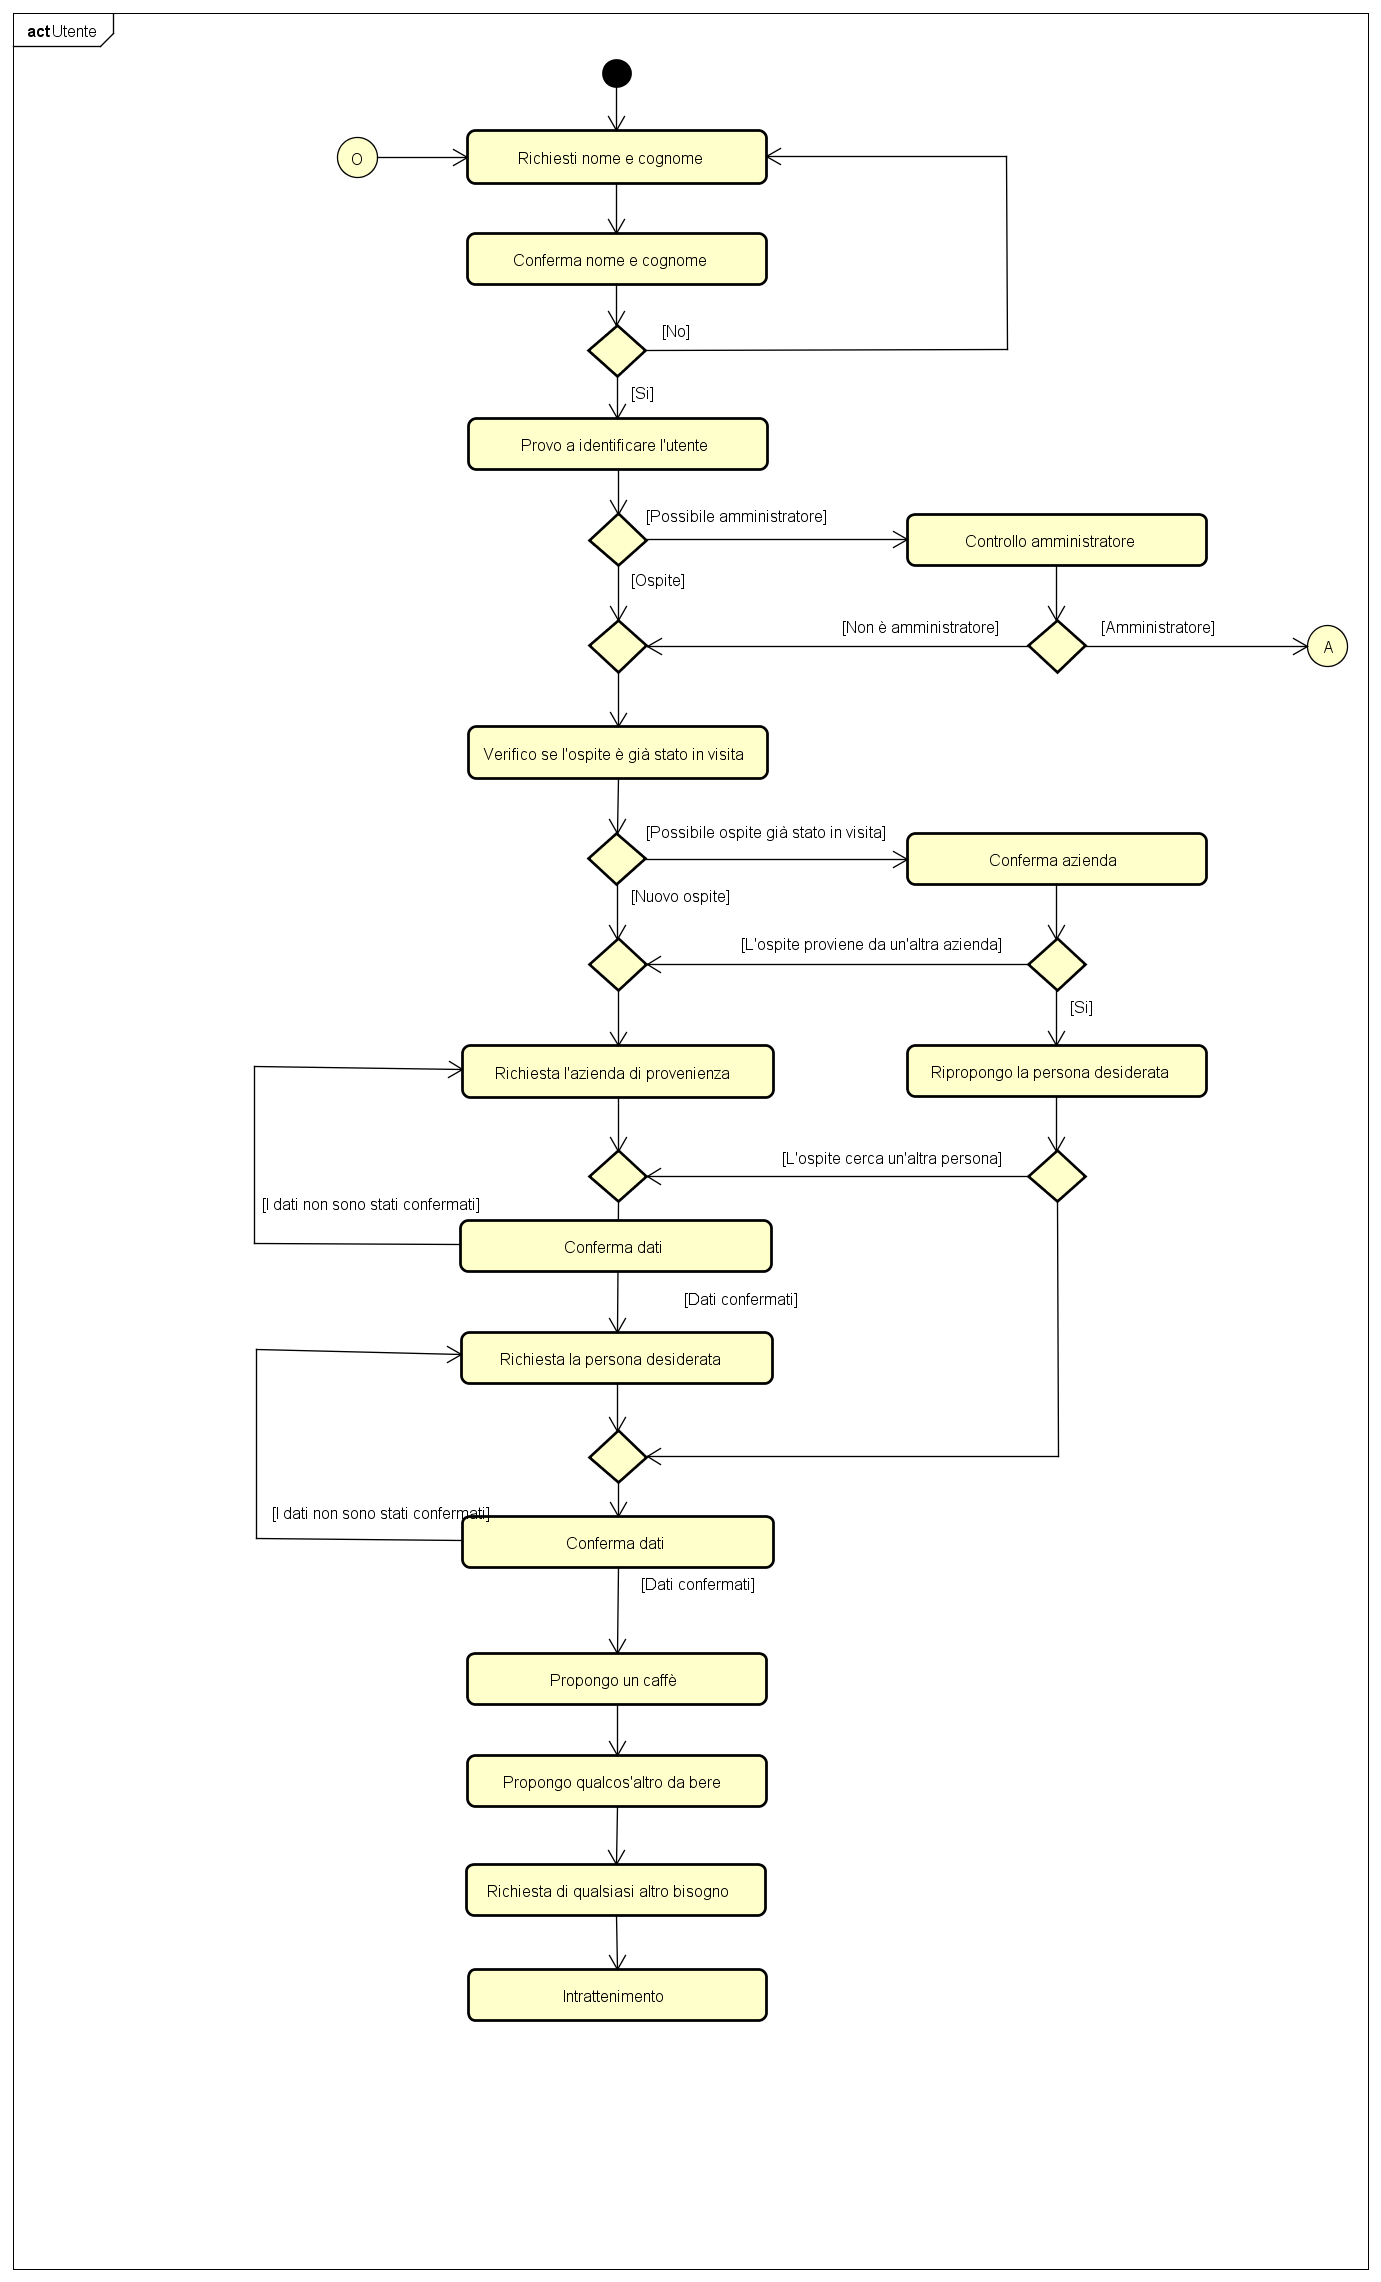
\includegraphics[width=0.7\textwidth,height=\textheight,keepaspectratio]{sezioni/images/Utente.png}}
	\caption{Flusso del dialogo per un ospite}\label{fig:flussoOspite}
\end{figure}
\newpage
\subsubsection{Amministratore}\label{admin}
Le funzionalità disponibili ad un amministratore del sistema sono le seguenti:
\begin{itemize}
	\item effettuare l'accesso all'area di amministrazione;
	\item aggiunta di una \gl{rule} (\gl{direttiva});
	\item rimozione di una rule;
	\item aggiornamento di una rule;
	\item lettura di una o più rule;
	\item aggiunta di un \gl{target};
	\item aggiornamento di un target;
	\item rimozione di un target;
	\item aggiornare i propri dati;
	\item lettura di uno o più amministratori.
\end{itemize}
\paragraph{Effettuare l'accesso all'area di amministrazione}\label{adminArea}
Solo gli utenti registrati possono effettuare l'accesso all'area di amministrazione. La registrazione di un nuovo amministratore è consentita solo al super amministratore del sistema, la quale procedura è spiegata in \ref{AddAdmin}. \\
Per effettuare l'accesso, seguire la seguente procedura:
\begin{itemize}
	\item esordire con un saluto (ad esempio "Hi", "Hello", "Good morning");
	\item \PROGETTO{} darà il benvenuto in azienda e chiederà il nome e il cognome dell'interlocutore. È importante che vengano forniti sia nome che cognome e non solo uno di essi;
	\item pronunciare nome e cognome;
	\item \PROGETTO, cercando nel database apposito, tenterà di capire se i dati forniti sono associati ad un amministratore esistente. Se sì, due scenari sono possibili:
	\begin{itemize}
		\item un solo amministratore esistente è associato ai dati forniti, \PROGETTO{} recupererà dal database l'username e chiederà conferma all'interlocutore;
		\item più amministratori sono associati ai dati forniti, \PROGETTO{} chiederà quindi che venga comunicato l'username dell'amministratore con il quale effettuare l'accesso. Successivamente, viene chiesta conferma; 
	\end{itemize}
	Altrimenti, l'interlocutore viene trattato come un ospite;
	\item se corretti, dare conferma dei dati recuperati da \PROGETTO, smentire altrimenti;
	\item pronunciare la frase di riconoscimento che \PROGETTO{} fornirà.
\end{itemize}
\paragraph{Aggiunta di una rule}
Per aggiungere una rule, seguire la seguente procedura:
\begin{itemize}
	\item pronunciare una frase del tipo "add rule" o "I want to add a rule";
	\item \PROGETTO{} chiederà di inserire un parametro per volta (nome della rule, \gl{task} e \gl{target});
	\item una volta raccolti, \PROGETTO{} chiederà la conferma dei dati;
	\item se si nega la conferma, si ritornerà al pannelo di amministrazione.
\end{itemize}
Alla voce \gl{task} nel glossario (\ref{task}) è presente l'elenco dei task supportati.
\paragraph{Rimozione di una rule}
Per rimuovere una rule, seguire la seguente procedura:
\begin{itemize}
	\item pronunciare una frase del tipo "remove rule" o "I want to remove a rule";
	\item \PROGETTO{} chiederà il nome della rule che si vuole eliminare;
	\item una volta raccolti, \PROGETTO{} chiederà la conferma dei dati;
	\item se si nega la conferma, si ritornerà al pannelo di amministrazione.
\end{itemize}
Questa operazione è possibile solo sulle rule definite dall'amministratore loggato.
\paragraph{Aggiornamento di una rule}
Per aggiornare una rule, seguire la seguente procedura:
\begin{itemize}
	\item pronunciare una frase del tipo "update rule" o "I want to update a rule";
	\item \PROGETTO{} chiederà il nome della rule che si vuole aggiornare;
	\item una volta raccolti, \PROGETTO{} chiederà la conferma dei dati;
	\item se si nega la conferma, si ritornerà al pannelo di amministrazione.
\end{itemize}
Vista la natura dell'input di tipo vocale, i \gl{target} di una rule devono essere aggiornati a parte, come spiegato in \ref{updateRuleTarget}.
Questa operazione è possibile solo sulle rule definite dall'amministratore loggato.
\paragraph{Lettura di una o più rule}
Per ottenere i dati di una rule, seguire la seguente procedura:
\begin{itemize}
	\item pronunciare una frase del tipo "get rule" o "I want to retrieve a rule";
	\item \PROGETTO{} chiederà il nome della rule che si vuole ottenere;
	\item se esistente, verrà restituita la relativa rule.
\end{itemize}

Per ottenere i dati di tutte le rule esistenti, pronunciare una frase del tipo "get all rule", "get rule list" o "retrieve all rules".
\paragraph{Aggiunta di un target}\label{addRuleTarget}
Per aggiungere un target ad una rule, seguire la seguente procedura:
\begin{itemize}
	\item pronunciare una frase del tipo "add rule target" o "I want to add a rule target";
	\item \PROGETTO{} chiederà il nome della rule nella quale aggiungere il target;
	\item \PROGETTO{} chiederà di pronunciare i parametri del nuovo target (nome, azienda di provenienza, \gl{member});
	\item una volta raccolti, \PROGETTO{} chiederà la conferma dei dati;
	\item se si nega la conferma, si ritornerà al pannello di amministrazione.
\end{itemize}
\paragraph{Rimozione di un target}
Per rimuovere un target da una rule, seguire la seguente procedura:
\begin{itemize}
	\item pronunciare una frase del tipo "remove rule target" o "I want to remove a rule target";
	\item \PROGETTO{} chiederà il nome della rule dalla quale rimuovere il target;
	\item \PROGETTO{} chiederà di pronunciare i parametri del target da rimovere (nome, azienda di provenienza, \gl{member});
	\item una volta raccolti, \PROGETTO{} chiederà la conferma dei dati;
	\item se si nega la conferma, si ritornerà al pannelo di amministrazione.
\end{itemize}
Questa operazione è possibile solo sulle rule definite dall'amministratore loggato.
\paragraph{Aggiornamento di un target}\label{updateRuleTarget}
Per aggiornare un target di una rule, seguire la seguente procedura:
\begin{itemize}
	\item pronunciare una frase del tipo "update rule target" o "I want to update a rule target";
	\item \PROGETTO{} chiederà il nome della rule nella quale aggiornare il target;
	\item \PROGETTO{} chiederà di pronunciare i parametri del target da aggiornare (nome, azienda di provenienza, \gl{member});
	\item una volta raccolti, \PROGETTO{} chiederà la conferma dei dati;
	\item se si nega la conferma, si ritornerà al pannelo di amministrazione.
\end{itemize}
Questa operazione è possibile solo sulle rule definite dall'amministratore loggato.
\paragraph{Aggiornamento dei propri dati}

Per aggiornare i propri dati, l'amministratore loggato deve seguire la seguente procedura:
\begin{itemize}
	\item pronunciare una frase del tipo "update data" o "I want to update my data";
	\item \PROGETTO{} chiederà i nuovi dati da aggiornare;
	\item una volta raccolti, \PROGETTO{} chiederà la conferma dei dati;
	\item se si nega la conferma, si ritornerà al pannelo di amministrazione.
\end{itemize}

\paragraph{Lettura di uno o più amministratori}
Per ottenere i dati di un amministratore, seguire la seguente procedura:
\begin{itemize}
	\item pronunciare una frase del tipo "get user" o "I want to retrieve a user";
	\item \PROGETTO{} chiederà il nome dell'amministratore che si vuole ottenere;
	\item se esistente, verrà restituito il relativo amministratore (dati sensibili esclusi).
\end{itemize}

Per ottenere i dati di tutti gli amministratori esistenti (dati sensibili esclusi), pronunciare una frase del tipo "get all users", "get users list" o "I want to retrieve all users".

\subsubsection{Super Amministratore}\label{superAdmin}
Un super amministratore è un amministratore con privilegi maggiori, in quanto può operare su tutti gli utenti del sistema e le rule indipendentemente da chi le abbia create, con anche un numero di funzionalità più grande rispetto agli amministratori.
Infatti, in caso un amministratore venga eliminato dal sistema (operazione possibile solo per il super amministratore), le rule da lui create non saranno eliminate, ma saranno comunque sotto il controllo del super amministratore. \\
Le funzionalità aggiuntive sono:
\begin{itemize}
	\item aggiunta di un amministratore;
	\item aggiornamento di un amministratore;
	\item rimozione di un amministratore;
	\item aggiunta dell'enrollment di un amministratore;
	\item rimozione dell'enrollment di un amministratore.
\end{itemize}
\paragraph{Aggiunta di un amministratore}\label{AddAdmin}
Per aggiungere un amministratore, seguire la seguente procedura:
\begin{itemize}
	\item pronunciare una frase del tipo "add admin" o "I want to add an admin";
	\item \PROGETTO{} chiederà il nome e il cognome del nuovo amministratore. È importante che vengano forniti sia nome che cognome e non solo uno di essi;
	\item \PROGETTO{} chiederà l'username del nuovo amministratore;
	\item una volta raccolti, \PROGETTO{} chiederà la conferma dei dati;
	\item se si nega la conferma, si ritornerà al \gl{pannello di amministrazione}.
\end{itemize}

Vista la natura dell'input di tipo vocale, l'\gl{enrollment} di un amministratore deve essere aggiunto a parte, come spiegato in \ref{addEnrollment}.
\paragraph{Aggiornamento di un amministratore}
 Per aggiornare un amministratore, seguire la seguente procedura:
\begin{itemize}
	\item pronunciare una frase del tipo "update admin" o "I want to update an admin";
	\item \PROGETTO{} chiederà l'username dell'amministratore che si vuole aggiornare;
	\item \PROGETTO{} chiederà l'inserimento dei nuovi dati;
	\item una volta raccolti, \PROGETTO{} chiederà la conferma dei dati;
	\item se si nega la conferma, si ritornerà al pannello di amministrazione.
\end{itemize}

\paragraph{Rimozione di un amministratore}
 Per rimuovere un amministratore, seguire la seguente procedura:
\begin{itemize}
	\item pronunciare una frase del tipo "remove admin" o "I want to remove an admin";
	\item \PROGETTO{} chiederà l'username dell'amministratore che si vuole rimuovere;
	\item una volta raccolti, \PROGETTO{} chiederà la conferma dei dati;
	\item se si nega la conferma, si ritornerà al pannello di amministrazione.
\end{itemize}

Quando un amministratore viene rimosso, le rule da lui create non vengono rimosse.
\paragraph{Aggiunta dell'enrollment di un amministratore}\label{addEnrollment}

Per aggiungere un enrollment ad un amministratore, per crearne quindi l'impronta vocale, è necessario seguire la seguente procedura:
\begin{itemize}
	\item pronunciare una frase del tipo "add enrollment" o "I want to add an enrollment";
	\item \PROGETTO{} chiederà l'username dell'amministratore al quale aggiungere l'enrollment;
	\item \PROGETTO{} mostrerà una frase la quale deve essere pronunciata dall'amministratore da aggiungere \textbf{in persona}; 
	\item una volta raccolti, \PROGETTO{} chiederà la conferma dei dati;
	\item se si nega la conferma, si ritornerà al pannello di amministrazione.
\end{itemize}
\paragraph{Reset dell'enrollment di un amministratore}

Per resettare l'enrollment di un amministratore, è necessario seguire la seguente procedura:
\begin{itemize}
	\item pronunciare una frase del tipo "reset enrollment" o "I want to reset an enrollment";
	\item \PROGETTO{} chiederà l'username dell'amministratore al quale resettare l'enrollment;
	\item una volta raccolti, \PROGETTO{} chiederà la conferma dei dati;
	\item se si nega la conferma, si ritornerà al pannello di amministrazione.
\end{itemize}
\section{Glossario}
\subsection*{Enrollment}
\subsection*{Member}
\subsection*{Rule (direttiva)}
\subsection*{Target}
\subsection*{Task}

\end{document}
